\documentclass[hyperref, a4paper]{report}

\usepackage{geometry}
\usepackage{titling}
\usepackage{titlesec}
% No longer needed, since we will use enumitem package
% \usepackage{paralist}
\usepackage{enumitem}
\usepackage{footnote}
\usepackage{amsmath, amssymb, amsthm}
\usepackage{mathtools}
\usepackage{bbm}
\usepackage{cite}
\usepackage{graphicx}
\usepackage{subfigure}
\usepackage{physics}
\usepackage{tensor}
\usepackage{siunitx}
\usepackage[version=4]{mhchem}
\usepackage{tikz}
\usepackage{xcolor}
\usepackage{listings}
\usepackage{underscore}
\usepackage{autobreak}
\usepackage[ruled, vlined, linesnumbered]{algorithm2e}
\usepackage{nameref,zref-xr}
\zxrsetup{toltxlabel}
\usepackage[colorlinks,unicode]{hyperref} % , linkcolor=black, anchorcolor=black, citecolor=black, urlcolor=black, filecolor=black
\usepackage[most]{tcolorbox}
\usepackage{prettyref}

% Page style
\geometry{left=3.18cm,right=3.18cm,top=2.54cm,bottom=2.54cm}
\titlespacing{\paragraph}{0pt}{1pt}{10pt}[20pt]
\setlength{\droptitle}{-5em}

% More compact lists 
\setlist[itemize]{
    %itemindent=17pt, 
    %leftmargin=1pt,
    listparindent=\parindent,
    parsep=0pt,
}

\setlist[enumerate]{
    %itemindent=17pt, 
    %leftmargin=1pt,
    listparindent=\parindent,
    parsep=0pt,
}

% Math operators
\DeclareMathOperator{\timeorder}{\mathcal{T}}
\DeclareMathOperator{\diag}{diag}
\DeclareMathOperator{\legpoly}{P}
\DeclareMathOperator{\primevalue}{P}
\DeclareMathOperator{\sgn}{sgn}
\DeclareMathOperator{\res}{Res}
\newcommand*{\ii}{\mathrm{i}}
\newcommand*{\ee}{\mathrm{e}}
\newcommand*{\const}{\mathrm{const}}
\newcommand*{\suchthat}{\quad \text{s.t.} \quad}
\newcommand*{\argmin}{\arg\min}
\newcommand*{\argmax}{\arg\max}
\newcommand*{\normalorder}[1]{: #1 :}
\newcommand*{\pair}[1]{\langle #1 \rangle}
\newcommand*{\fd}[1]{\mathcal{D} #1}
\DeclareMathOperator{\bigO}{\mathcal{O}}

% TikZ setting
\usetikzlibrary{arrows,shapes,positioning}
\usetikzlibrary{arrows.meta}
\usetikzlibrary{decorations.markings}
\usetikzlibrary{calc}
\tikzstyle arrowstyle=[scale=1]
\tikzstyle directed=[postaction={decorate,decoration={markings,
    mark=at position .5 with {\arrow[arrowstyle]{stealth}}}}]
\tikzstyle ray=[directed, thick]
\tikzstyle dot=[anchor=base,fill,circle,inner sep=1pt]

% Algorithm setting
% Julia-style code
\SetKwIF{If}{ElseIf}{Else}{if}{}{elseif}{else}{end}
\SetKwFor{For}{for}{}{end}
\SetKwFor{While}{while}{}{end}
\SetKwProg{Function}{function}{}{end}
\SetArgSty{textnormal}

\newcommand*{\concept}[1]{{\textbf{#1}}}

% Embedded codes
\lstset{basicstyle=\ttfamily,
  showstringspaces=false,
  commentstyle=\color{gray},
  keywordstyle=\color{blue}
}

\lstdefinestyle{console}{
    basicstyle=\footnotesize\ttfamily,
    breaklines=true,
    postbreak=\mbox{\textcolor{red}{$\hookrightarrow$}\space}
}

% Reference formatting
\newrefformat{fig}{Figure~\ref{#1}}

% Color boxes
\tcbuselibrary{skins, breakable, theorems}
\newtcbtheorem[number within=section]{warning}{Warning}%
  {colback=orange!5,colframe=orange!65,fonttitle=\bfseries, breakable}{warn}
\newtcbtheorem[number within=section]{note}{Note}%
  {colback=green!5,colframe=green!65,fonttitle=\bfseries, breakable}{note}
\newtcbtheorem[number within=section]{info}{Info}%
  {colback=blue!5,colframe=blue!65,fonttitle=\bfseries, breakable}{info}

% Displaying texts in bookmarkers

\pdfstringdefDisableCommands{%
  \def\\{}%
  \def\ce#1{<#1>}%
}

\pdfstringdefDisableCommands{%
  \def\texttt#1{<#1>}%
  \def\mathbb#1{#1}%
}
\pdfstringdefDisableCommands{\def\eqref#1{(\ref{#1})}}

\makeatletter
\pdfstringdefDisableCommands{\let\HyPsd@CatcodeWarning\@gobble}
\makeatother

\newenvironment{shelldisplay}{\begin{lstlisting}}{\end{lstlisting}}

\newcommand{\shortcode}[1]{\texttt{#1}}

\lstset{style = console}

% Make subsubsection labeled
\setcounter{secnumdepth}{4}
\setcounter{tocdepth}{4}


\title{Manual for DFT+$GW$+BSE and the related matters}
\author{Jinyuan Wu}

\begin{document}
    
\maketitle

\chapter{$GW$ and BSE}

\section{Preliminaries}

\subsection{Details in diagrammatics}

This section briefly goes through some tricky aspects of Feynman diagram techniques 
that may seem puzzling when we do concrete calculations.

\subsubsection{Infinitesimals}

Note that here we need to add some convergence factors.
The first is about the value of the propagator 
to ensure that when $t = 0$, $\timeorder \expval*{c(t) c^\dagger(0)}$ is the particle number 
(so that if we evaluate the tadpole diagram, 
we get the Hartree term), 
the contribution of an electron line is actually 
\begin{equation}
    \begin{aligned}
        \timeorder \expval*{c_{\vb*{k}}(t) c_{\vb*{k}}^\dagger(0)} 
        &\coloneqq 
        \timeorder \expval*{c_{\vb*{k}}(t - 0^+) c_{\vb*{k}}^\dagger(0)}  \\
        &= \int \frac{\dd{\omega}}{2\pi} \ee^{- \ii \omega (t - 0^+)} 
        \underbrace{
            \frac{\ii}{\omega - \xi_{\vb*{k}} + \ii 0^+ \sgn(\xi_{\vb*{k}})}
        }_{\ii G_0(\omega, \vb*{k})}
        = \int \frac{\dd{\omega}}{2\pi} \ee^{- \ii \omega t} \ee^{\ii \omega 0^+} \ii G_0(\omega, \vb*{k}) .
    \end{aligned} 
\end{equation}
The necessity of this $\ee^{\ii \omega 0^+}$ factor 
can also be seen by explicitly doing the integration:
when $t = 0$, if we ignore the $\ee^{\ii \omega 0^+}$ factor, 
we get 
\[
    \int \frac{\dd{\omega}}{2\pi} \frac{\ii}{ \omega - \xi_{\vb*{k}} + \ii 0^+ \sgn(\xi_{\vb*{k}})}.
\]
This integral is not zero, but we want it to be zero when $\xi_{\vb*{k}} > 0$,
so we have to add a $\ee^{\ii \omega 0^+}$ factor
to make the integrand approaches zero quickly enough in the upper plane,
so we can construct an integration contour in the upper plane,
in which there is no pole, 
and 
\[
    \int_{\abs{\omega} = R \gg 1} \frac{\dd{\omega}}{2\pi} 
    \frac{\ii}{ \omega - \xi_{\vb*{k}} + \ii 0^+ \sgn(\xi_{\vb*{k}})} = 0.
\]

Another mini-regularization is when necessary, 
for a real space interaction line -- screened or unscreened -- 
we should assume the ``out-time'' is the ``in-time'' plus $0^+$,
because the Coulomb interaction isn't really spontaneous
and there is a small time retardation.
In the frequency space,
we need to assume that there is an infinite amount of energy on the interaction line,

For bare Coulomb interaction this is rarely needed,
because we don't have $\omega$ dependence in the potential,
and it makes no sense to discuss the poles when we change $\omega$.
It does make sense to talk about retardation 
in the relativistic origin of Coulomb interaction:
the Coulomb interaction is mediated by virtual photons,
and is therefore proportional to the off-shell (i.e. $\omega \to 0$) limit of 
the photon propagator, 
which has $\omega^2 - \vb*{q}^2 + \ii 0^+$ 
as the denominator, and we get 
\begin{equation}
    V(q) = \frac{4\pi e^2}{\vb*{q}^2 - \omega^2 - \ii 0^+}.
    \label{eq:v-light-rel}
\end{equation}

For screened Coulomb interaction, however, 
the correct retardation is important,
because now something looking like \eqref{eq:v-light-rel} appears again.

\subsubsection{The position of imaginary units}

In this section I only consider how many imaginary units there are in front of 
Green functions, self energies, etc.
Normalization factors like $2\pi$ or $V$ 
involved in summation of $\vb*{r}$ or $\vb*{k}$ are not considered.

The self-energy correction is visualized as the follows:
\begin{equation}
    - \Sigma^{\text{Hartree}}_{\vb*{k} \sigma \omega} = \begin{gathered}
        \begin{tikzpicture}[x=0.75pt,y=0.75pt,yscale=-1,xscale=1]
            %uncomment if require: \path (0,300); %set diagram left start at 0, and has height of 300
            
            %Straight Lines [id:da7796585827567135] 
            \draw  [dash pattern={on 4.5pt off 4.5pt}]  (247.35,162.98) -- (247.35,211) ;
            %Shape: Circle [id:dp5603225998122126] 
            \draw   (218.35,133.98) .. controls (218.35,117.96) and (231.34,104.98) .. (247.35,104.98) .. controls (263.37,104.98) and (276.35,117.96) .. (276.35,133.98) .. controls (276.35,150) and (263.37,162.98) .. (247.35,162.98) .. controls (231.34,162.98) and (218.35,150) .. (218.35,133.98) -- cycle ;
            %Straight Lines [id:da24340217870718206] 
            \draw    (254.35,105.98) ;
            \draw [shift={(254.35,105.98)}, rotate = 180] [fill={rgb, 255:red, 0; green, 0; blue, 0 }  ][line width=0.08]  [draw opacity=0] (12,-3) -- (0,0) -- (12,3) -- cycle    ;
            
            % Text Node
            \draw (217,83.4) node [anchor=north west][inner sep=0.75pt]    {$\boldsymbol{k} ',\alpha ,0$};
            \end{tikzpicture}      
   \end{gathered} = \frac{1}{V} \sum_{\vb*{k}', \alpha} (- V_0) n_{\vb*{k}' \alpha}^0,
   \label{eq:lowerest-self-energy-hartree-fermi-liquid}
\end{equation}
and from it we have 
\[
    \ii G= \ii G_{0} + \ii G_{0} \ii G\times \tikzset{every picture/.style={line width=0.75pt}} %set default line width to 0.75pt        
\begin{tikzpicture}[x=0.75pt,y=0.75pt,yscale=-1,xscale=1, baseline=(XXXX.south) ]
\path (0,75);\path (56,0);\draw    ($(current bounding box.center)+(0,0.3em)$) node [anchor=south] (XXXX) {};
%Shape: Circle [id:dp046942194255674474] 
\draw  [fill={rgb, 255:red, 155; green, 155; blue, 155 }  ,fill opacity=1 ] (8.54,37.54) .. controls (8.54,27.35) and (16.81,19.08) .. (27,19.08) .. controls (37.19,19.08) and (45.46,27.35) .. (45.46,37.54) .. controls (45.46,47.74) and (37.19,56) .. (27,56) .. controls (16.81,56) and (8.54,47.74) .. (8.54,37.54) -- cycle ;
\end{tikzpicture}.
\]
It's then a good idea to define 
\begin{equation}
    -\ii \Sigma =\tikzset{every picture/.style={line width=0.75pt}} %set default line width to 0.75pt        
    \begin{tikzpicture}[x=0.75pt,y=0.75pt,yscale=-1,xscale=1, baseline=(XXXX.south) ]
    \path (0,75);\path (56,0);\draw    ($(current bounding box.center)+(0,0.3em)$) node [anchor=south] (XXXX) {};
    %Shape: Circle [id:dp046942194255674474] 
    \draw  [fill={rgb, 255:red, 155; green, 155; blue, 155 }  ,fill opacity=1 ] (8.54,37.54) .. controls (8.54,27.35) and (16.81,19.08) .. (27,19.08) .. controls (37.19,19.08) and (45.46,27.35) .. (45.46,37.54) .. controls (45.46,47.74) and (37.19,56) .. (27,56) .. controls (16.81,56) and (8.54,47.74) .. (8.54,37.54) -- cycle ;
    \end{tikzpicture},
\end{equation}
because in this case, we have 
\begin{equation}
    G = G_0 + G G_0 \Sigma,
\end{equation}
and therefore 
\begin{equation}
    \underbrace{\omega - \xi^0_{\vb*{k}}}_{{1}/{G_0}} = \underbrace{\omega - \xi_{\vb*{k}}}_{1 / G} + \Sigma,
\end{equation}
which agrees with the definition of the self energy as the shift of single-particle energy from the free dispersion.

Similarly, we define the corrected interaction line as 
\begin{equation}
    -\ii W=\tikzset{every picture/.style={line width=0.75pt}} %set default line width to 0.75pt        
    \begin{tikzpicture}[x=0.75pt,y=0.75pt,yscale=-1,xscale=1, baseline=(XXXX.south) ]
    \path (0,75);\path (32,0);\draw    ($(current bounding box.center)+(0,0.3em)$) node [anchor=south] (XXXX) {};
    %Straight Lines [id:da583204631520762] 
    \draw    (14.5,62.99) .. controls (12.85,61.3) and (12.87,59.64) .. (14.55,57.99) .. controls (16.23,56.34) and (16.24,54.67) .. (14.59,52.99) .. controls (12.94,51.31) and (12.96,49.64) .. (14.64,47.99) .. controls (16.32,46.34) and (16.33,44.67) .. (14.68,42.99) .. controls (13.03,41.31) and (13.05,39.64) .. (14.73,37.99) .. controls (16.41,36.34) and (16.43,34.67) .. (14.78,32.99) .. controls (13.13,31.31) and (13.14,29.64) .. (14.82,27.99) .. controls (16.5,26.34) and (16.52,24.67) .. (14.87,22.99) .. controls (13.22,21.31) and (13.24,19.64) .. (14.92,17.99) -- (14.94,15.59) -- (14.94,15.59)(17.5,63.01) .. controls (15.85,61.33) and (15.87,59.66) .. (17.55,58.01) .. controls (19.23,56.36) and (19.24,54.69) .. (17.59,53.01) .. controls (15.94,51.33) and (15.96,49.66) .. (17.64,48.01) .. controls (19.32,46.36) and (19.33,44.69) .. (17.68,43.01) .. controls (16.03,41.33) and (16.05,39.66) .. (17.73,38.01) .. controls (19.41,36.36) and (19.43,34.7) .. (17.78,33.02) .. controls (16.13,31.34) and (16.14,29.67) .. (17.82,28.02) .. controls (19.5,26.37) and (19.52,24.7) .. (17.87,23.02) .. controls (16.22,21.34) and (16.24,19.67) .. (17.92,18.02) -- (17.94,15.62) -- (17.94,15.62) ;
    \end{tikzpicture},
\end{equation}
because in this way, when there is no interaction corrections,
we have 
\begin{equation}
    W = \frac{e^2}{r} \eqqcolon v.
\end{equation}

\subsubsection{About ``antiparticles''}

The directions of momentum lines indicate whether the particles are created or annihilated.
When the momentum arrow goes against the arrow on a line,
we say this line is an antiparticle line.
But here is a puzzle:
we know there is no such thing as positrons in condensed matter physics,
so what does ``antiparticle'' mean?

Here the problem lies on what it means to be the antiparticle of a kind of particle.
In particle physics,
when we do the particle-antiparticle transformation to an electron state 
whose polarization is one of the Dirac basis,
a $\psi^+$ particle is flipped into a $\psi^-$ particle and vice versa.
In condensed matter physics, the label of $\psi^+$ and $\psi^-$
(or $\phi$ and $\chi$ as people often call them:
$\psi = (\phi, \chi)$) is no longer there:
the $\chi$ modes in the Dirac field have already been integrated out.
So electrons in condensed matter physics don't really have antiparticles 
in the context of high energy physics.

Indeed, if we are still dealing with scattering problems in the non-relativistic limit,
the antiparticle lines don't appear at all!
And similar to the case in QED (which can be checked in Peskin (A.6)), 
no separate momentum arrows parallel to the internal lines are needed:
When calculating the propagator, 
the processes of both ``an electron traveling forward'' and ``a hole traveling backward''
are automatically covered together.

The antiparticle lines only appear when there are electrons in the ground state,
which usually indicates there is a $-\mu N$ term in the Hamiltonian
so having some preexisting electrons lower the energy further,
and this differs with the scattering case only in the rules pertaining to the external lines.
For external lines, we now have diagrams like the following:
\[
\begin{gathered}
    \begin{tikzpicture}[x=0.75pt,y=0.75pt,yscale=-0.8,xscale=0.8]
        %uncomment if require: \path (0,300); %set diagram left start at 0, and has height of 300
        
        %Straight Lines [id:da22337196735465925] 
        \draw    (59,160) .. controls (60.67,158.33) and (62.33,158.33) .. (64,160) .. controls (65.67,161.67) and (67.33,161.67) .. (69,160) .. controls (70.67,158.33) and (72.33,158.33) .. (74,160) .. controls (75.67,161.67) and (77.33,161.67) .. (79,160) .. controls (80.67,158.33) and (82.33,158.33) .. (84,160) .. controls (85.67,161.67) and (87.33,161.67) .. (89,160) .. controls (90.67,158.33) and (92.33,158.33) .. (94,160) .. controls (95.67,161.67) and (97.33,161.67) .. (99,160) .. controls (100.67,158.33) and (102.33,158.33) .. (104,160) .. controls (105.67,161.67) and (107.33,161.67) .. (109,160) -- (112,160) -- (112,160) ;
        %Straight Lines [id:da2810352455475442] 
        \draw    (112,160) -- (154,115.21) ;
        \draw [shift={(137.79,132.5)}, rotate = 133.16] [fill={rgb, 255:red, 0; green, 0; blue, 0 }  ][line width=0.08]  [draw opacity=0] (12,-3) -- (0,0) -- (12,3) -- cycle    ;
        %Straight Lines [id:da3072568651468959] 
        \draw    (154,206.21) -- (112,160) ;
        \draw [shift={(128.29,177.92)}, rotate = 47.73] [fill={rgb, 255:red, 0; green, 0; blue, 0 }  ][line width=0.08]  [draw opacity=0] (12,-3) -- (0,0) -- (12,3) -- cycle    ;
        %Straight Lines [id:da8519748557010314] 
        \draw    (111,146) -- (135.61,120.64) ;
        \draw [shift={(137,119.21)}, rotate = 134.14] [fill={rgb, 255:red, 0; green, 0; blue, 0 }  ][line width=0.08]  [draw opacity=0] (12,-3) -- (0,0) -- (12,3) -- cycle    ;
        %Straight Lines [id:da18850975613378163] 
        \draw    (111,173) -- (133.65,197.73) ;
        \draw [shift={(135,199.21)}, rotate = 227.52] [fill={rgb, 255:red, 0; green, 0; blue, 0 }  ][line width=0.08]  [draw opacity=0] (12,-3) -- (0,0) -- (12,3) -- cycle    ;
        %Straight Lines [id:da6750821989366331] 
        \draw    (214,160) .. controls (215.67,158.33) and (217.33,158.33) .. (219,160) .. controls (220.67,161.67) and (222.33,161.67) .. (224,160) .. controls (225.67,158.33) and (227.33,158.33) .. (229,160) .. controls (230.67,161.67) and (232.33,161.67) .. (234,160) .. controls (235.67,158.33) and (237.33,158.33) .. (239,160) .. controls (240.67,161.67) and (242.33,161.67) .. (244,160) .. controls (245.67,158.33) and (247.33,158.33) .. (249,160) .. controls (250.67,161.67) and (252.33,161.67) .. (254,160) .. controls (255.67,158.33) and (257.33,158.33) .. (259,160) .. controls (260.67,161.67) and (262.33,161.67) .. (264,160) -- (267,160) -- (267,160) ;
        %Straight Lines [id:da7852623112527173] 
        \draw    (267,160) -- (309,115.21) ;
        \draw [shift={(292.79,132.5)}, rotate = 133.16] [fill={rgb, 255:red, 0; green, 0; blue, 0 }  ][line width=0.08]  [draw opacity=0] (12,-3) -- (0,0) -- (12,3) -- cycle    ;
        %Straight Lines [id:da940793106803989] 
        \draw    (309,206.21) -- (267,160) ;
        \draw [shift={(283.29,177.92)}, rotate = 47.73] [fill={rgb, 255:red, 0; green, 0; blue, 0 }  ][line width=0.08]  [draw opacity=0] (12,-3) -- (0,0) -- (12,3) -- cycle    ;
        %Straight Lines [id:da5232058447471666] 
        \draw    (266,146) -- (290.61,120.64) ;
        \draw [shift={(292,119.21)}, rotate = 134.14] [fill={rgb, 255:red, 0; green, 0; blue, 0 }  ][line width=0.08]  [draw opacity=0] (12,-3) -- (0,0) -- (12,3) -- cycle    ;
        %Straight Lines [id:da3253102481261483] 
        \draw    (267.35,174.47) -- (290,199.21) ;
        \draw [shift={(266,173)}, rotate = 47.52] [fill={rgb, 255:red, 0; green, 0; blue, 0 }  ][line width=0.08]  [draw opacity=0] (12,-3) -- (0,0) -- (12,3) -- cycle    ;
        \end{tikzpicture}
\end{gathered},
\]%
because now it's possible to annihilate a preexisting electron in the ground state,
but for internal lines, momentum labels can still be directly attached to the internal lines.
This can be also seen by reckoning how Feynman rules are derived:
the series we obtain by expanding $\ee^{- \ii H t}$ 
contains field operators, not single creation or annihilation operators,
and after Wick expansion,
the correlation functions we get are all like $\expval*{\bar{\psi} \psi}$,
and of course an annihilation operator appearing 
in the expression of the out state in terms of the ground state 
can be contracted with a creative operator in $\ee^{- \ii H t}$,
and this is visualized as an ``antiparticle'' external line 
with an outward momentum line.
So here, the ``particle-antiparticle transformation''
is just swapping $c_{\vb*{k}}$ and $c_{\vb*{k}}^\dagger$
-- this operation is still legit in condensed matter physics,
because it doesn't involve the $\chi$ field;
of course, the operation doesn't create that kind of antiparticle in high energy physics.

No real modification happens to the propagator when there are electrons in the ground state. 
We have 
\begin{equation}
    \int_{-\infty}^\infty \ee^{\ii \omega t} \dd{t} \timeorder \expval*{c_{\vb*{k}}(t) c^\dagger(0)} = 
    \frac{\ii}{\omega - \epsilon_{\vb*{k}} + \mu},
\end{equation}
which can be straightforwardly obtained by looking at 
\begin{equation}
    H = \sum_{\vb*{k}} \epsilon_{\vb*{k}} c^\dagger_{\vb*{k}} c_{\vb*{k}} - \mu N
\end{equation}
without doing any calculation.

Now we have to face the tough question:
if antiparticle lines are there when there is a Fermi ball in the ground state,
then why poles corresponding to antiparticles (whatever they are) are absent in the propagator?
The answer is, for a $\vb*{k}$ on an antiparticle line appearing in diagrams,
the corresponding pole can indeed be understood as 
a pole of an antiparticle:
for an antiparticle line with momentum $\vb*{k}$,
$\vb*{k}$ has to be under the Fermi surface in the ground state,
so $\omega_{\vb*{k}} = \epsilon_{\vb*{k}} - \mu < 0$,
and the point $\omega = \omega_{\vb*{k}}$ thus may be understood as an antiparticle pole.
But here is a rather strong antisymmetry between particles and antiparticles: 
in external lines,
when particles appear ($\vb*{k}$ over Fermi surface),
antiparticles never appear; 
when antiparticles appear ($\vb*{k}$ below Fermi surface),
particles never appear.
The spectrum of electrons is split into two halves:
for the part over the Fermi surface,
only particles are visible,
while for the part below the Fermi surface,
only antiparticles are visible.

This means we can do away with antiparticle lines.
By defining 
\begin{equation}
    b_{\vb*{k}} = \begin{cases}
        c_{\vb*{k}}, &\quad \epsilon_{\vb*{k}} > \mu, \\
        c^\dagger_{\vb*{k}}, &\quad \epsilon_{\vb*{k}} < \mu,
    \end{cases}
\end{equation}
for $\epsilon_{\vb*{k}} < \mu$, we have
\begin{equation}
    \int_{-\infty}^\infty \ee^{\ii \omega t} \dd{t} \timeorder \expval*{b_{\vb*{k}}(t) b^\dagger(0)} 
    = \frac{\ii}{\omega - \mu + \epsilon_{\vb*{k}}},
\end{equation}
and now all poles have positive energies.
It's also easy to replace $c$ operators in all interaction vertices with $b$ operators,
so now, in the theory in terms of $b$ operators,
there is no antiparticle poles or Feynman diagrammatic antiparticle lines.
Indeed, $b$ operators give the true free excitation spectrum in a system with a non-zero chemical potential.

For $\epsilon_{\vb*{k}} < \mu$, $b_{\vb*{k}}^\dagger$ is said to \emph{create} a \concept{hole}.
The energy of a hole is still positive:
the energy of a state with a hole with momentum $\vb*{k}$
is 
\[
    \sum_{\vb*{k}' \neq \vb*{k}, \epsilon_{\vb*{k}'} < \mu} \epsilon_{\vb*{k}'} - \mu (N - 1),
\]
and compared with the ground state, the energy of the hole is 
\begin{equation}
    \begin{aligned}
        E &= \sum_{\vb*{k}' \neq \vb*{k}, \epsilon_{\vb*{k}'} < \mu} \epsilon_{\vb*{k}'} - \mu (N - 1) 
        - \left( \sum_{\epsilon_{\vb*{k}'} < \mu} \epsilon_{\vb*{k}'} - \mu N \right) \\
        &= \mu - \epsilon_{\vb*{k}} > 0.
    \end{aligned}
\end{equation}
So, we may say a hole is the antiparticle of an electron,
but when we talk about the former, 
the latter is just a part of the background.
Unlike the case in particle physics,
where the electron and the positron are definitely two things,
the hole and the electron are basically two \emph{representations} of the \emph{same} thing.
(But this doesn't make talking about ``annihilation between an electron and a hole'' nonsense,
because in an annihilation-between-electron-and-hole process,
the $n$ and $\vb*{k}$ numbers of the electron and the hole are different,
so there is no problem of double counting the same mode in two representations, etc.)

\subsubsection{Normalization}

\begin{equation}
    \int_{-\infty}^\infty \ee^{\ii \omega t} \dd{t} 
\end{equation}

\subsection{Feynman rules for actual calculation}

\subsubsection{In the free space}\label{sec:free-space}

TODO: $n$ interaction line $\Rightarrow$ $n$ independent momenta,
not all of which are on Coulomb interaction lines

A large benefit of this formalism
is it lifts the burden to worry about normalization concerning $\delta$-functions:
no $\delta$-function appears in the rules now!

\begin{equation}
    v(\vb*{q}) = \frac{4\pi e^2}{\vb*{q}^2}.
\end{equation}

\subsubsection{In a crystal}\label{sec:crystal}

There are several things that need attention concerning Feynman rules in condensed physics:
\begin{itemize}
    \item The propagator is no longer $1 / (\omega - \vb*{k}^2 / 2m)$, but 
    $\propto \sum_{\vb*{k}} \psi_{n \vb*{k}}(\vb*{r}) \psi^*_{n \vb*{k}} (\vb*{r}') / (\omega - \xi_{n \vb*{k}})$;
    \item The crystal momentum $\vb*{k}$ appears above. 
    To carry out Feynman diagrammatic calculations in an actual computer,
    a cutoff on the density of $\vb*{k}$ points is needed
    (essentially, a cutoff on the size of the system $V$).
    This means we should replace $\int \dd[3]{\vb*{k}} / 2\pi $
    with properly normalized $\sum_{\vb*{k}}$,
    where $\vb*{k}$ goes over the discretely infinite $\vb*{k}$-grid.
    \item Usually we limit all momenta to the \concept{first Brillouin zone (1BZ)}, 
    and therefore a sum over an unbounded momentum variable $\vb*{k}$ or $\vb*{q}$
    has to be recast into $\sum_{\vb*{G}} \sum_{\vb*{k}} f(\vb*{k} + \vb*{G})$.
\end{itemize}

Below I describe a set of Feynman rules that are compatible with the notation in \cite{hybertsen1986electron}.
Note that there is no controversy over 
normalization in the \emph{real space} Feynman diagrams:
although the inner structure of $G(1, 2)$ has changed in the presence of the crystal potential, 
its relation with other diagrammatic components as abstract entities 
is never changed.
Thus, starting from the space-in-real-space-and-time-in-frequency-space formalism may be a good idea:
the free-space momentum formalism 
however is an important reference for normalization constants.
In the space-in-real-space-and-time-in-frequency-space formalism,
in a diagram containing $n$ Coulomb interaction lines,
the variables summed over are $n$ frequency variables,
and $2n$ space variables,
and we just need to do 
\begin{equation}
    \int \frac{\dd{\omega}_1}{2\pi} \cdots \int \frac{\dd{\omega}_n}{2\pi} 
    \int \dd[3]{\vb*{r}_1} \cdots \int \dd[3]{\vb*{r}_{2n}}.
\end{equation}

We choose a normalization scheme for $\psi_{n \vb*{k}}$ such that 
\begin{equation}
    c^\dagger_{n \vb*{k}} = \int \dd[3]{\vb*{r}} 
    \underbrace{\ee^{\ii \vb*{k} \cdot \vb*{r}} u_{n \vb*{k}}(\vb*{r})}_{\psi_{n \vb*{k}}} 
    \psi^\dagger(\vb*{r}),
    \quad \acomm*{c_{n \vb*{k}}}{c^\dagger_{n' \vb*{k}'}} = \delta_{n n'} \delta_{\vb*{k} \vb*{k}'},
\end{equation}
where $\psi^\dagger(\vb*{r})$ is the complex conjugate 
of the non-relativistic electron field operator.
This leads to the normalization condition 
\begin{equation}
    \int \dd[3]{\vb*{r}} \psi^*_{n \vb*{k}}(\vb*{r}) \psi_{n' \vb*{k}'}(\vb*{r}) 
    = \delta_{n n'} \delta_{\vb*{k} \vb*{k}'},
    \label{eq:orthogonal}
\end{equation}
and
\begin{equation}
    G^0(\vb*{r}, \vb*{r}', \omega) = \sum_{n, \vb*{k}} \frac{
        \psi_{n \vb*{k}}(\vb*{r}) \psi^*_{n \vb*{k}}(\vb*{r}')
    }{\omega - \xi_{n \vb*{k}} + \ii 0^+ \sgn(\omega)}.
    \label{eq:green}
\end{equation}
In the free-electron case, 
we expect 
\begin{equation}
    \psi_{n \vb*{k}}(\vb*{r}) = \frac{1}{\sqrt{V}} \ee^{\ii (\vb*{k} + \vb*{G}_n) \cdot \vb*{r}},
\end{equation}
and therefore (note that the only possibility for $\vb*{G}_n + \vb*{k}$
to be equal to $\vb*{G}_{n'} + \vb*{k}'$
is for $\vb*{G}_n$ to be $\vb*{G}_{n'}$
and $\vb*{k}$ to be $\vb*{k}'$)
\[
    \text{LHS of \eqref{eq:orthogonal}} = 
    \frac{1}{V} \int \dd[3]{\vb*{r}} \ee^{\ii \vb*{r} (
        - \vb*{G}_n - \vb*{k} + \vb*{G}_{n'} + \vb*{k}'
    )} = 
    \frac{1}{V} V \delta_{\vb*{G}_n + \vb*{k}, \vb*{G}_{n'} + \vb*{k}'} 
    = \delta_{n n'} \delta_{\vb*{k} \vb*{k}'},
\]
and 
\[
    \begin{aligned}
        \text{RHS of \eqref{eq:green}} &= 
        \frac{1}{V} \sum_{n, \vb*{k}} 
        \ee^{\ii (\vb*{k} + \vb*{G}_n) \cdot (\vb*{r} - \vb*{r}')} 
        = \frac{1}{V} \sum_{\text{unbounded $\vb*{k}$}} 
        \ee^{\ii \vb*{k} \cdot (\vb*{r} - \vb*{r}')} \\
        &= \int \frac{\dd[3]{\vb*{k}}}{(2\pi)^3}
        \ee^{\ii \vb*{k} \cdot (\vb*{r} - \vb*{r}')}
        \eqqcolon \text{LHS of \eqref{eq:green}}, 
    \end{aligned}
\]
so \eqref{eq:orthogonal} and \eqref{eq:green}
go back to the free-space case.

Now we consider what happens when we encounter a Coulomb interaction line.
The structure in which a Coulomb interaction line is connected to four electron lines 
gives rise to the following factor in the interpretation of the diagram:
\begin{equation}
    M = \int \dd[3]{\vb*{r}} \int \dd[3]{\vb*{r}'}
    \ii G(\vb*{r}_4, \vb*{r}, \omega_1) \ii G(\vb*{r}_3, \vb*{r}', \omega_2)
    \ii G(\vb*{r}', \vb*{r}_2, \omega_3) \ii G(\vb*{r}, \vb*{r}_1, \omega_4)
    (- \ii) v(\vb*{r} - \vb*{r}').
\end{equation}
Note that here $\omega_4$ is just a shorthand of $\omega_1 + \omega_2 - \omega_3$
and this condition is \emph{not} imposed by a $\delta$-function factor
according to the rules listed above for the free-space case
(if we want to make this expression really symmetric, 
we should add a $2\pi \delta(\sum \omega)$ factor,
and let, say, $\int \dd{\omega_4} / 2\pi $ explicitly 
impose the energy conservation condition for us).
Inserting \eqref{eq:green} into the above expression,
and using the definition 
\begin{equation}
    v(\vb*{r} - \vb*{r}') = \int \frac{\dd[3]{\vb*{p}}}{(2\pi)^3} 
    \ee^{\ii \vb*{p} \cdot (\vb*{r} - \vb*{r}')} v(\vb*{p}),
\end{equation}
we have 
\begin{equation}
    \begin{aligned}
        M &= \psi_4(\vb*{r}_4) \psi_3(\vb*{r}_3) \psi_2^*(\vb*{r}_2) \psi_1^*(\vb*{r}_1) \\
        &\quad\quad \times 
        \int \frac{\dd[3]{\vb*{q}}}{(2\pi)^3} 
        \sum_{1, 2, 3, 4}
        \frac{\ii}{\omega_1 - \xi_4 + \ii 0^+ \sgn(\omega_1)}
        \frac{\ii}{\omega_1 - \xi_3 + \ii 0^+ \sgn(\omega_2)} \\
        &\quad\quad\quad \times 
        \frac{\ii}{\omega_1 - \xi_2 + \ii 0^+ \sgn(\omega_3)}
        \frac{\ii}{\omega_1 - \xi_1 + \ii 0^+ \sgn(\omega_4)} \\
        &\quad\quad\quad \times
        \int \dd[3]{\vb*{r}}  \psi_4^*(\vb*{r})  \psi_1(\vb*{r})  \ee^{\ii \vb*{q} \cdot \vb*{r}}
        \int \dd[3]{\vb*{r}'} \psi_3^*(\vb*{r}') \psi_2(\vb*{r}') \ee^{- \ii \vb*{q} \cdot \vb*{r}'}
        v(\vb*{q}),
    \end{aligned}
\end{equation}
where the label 1, 2, etc. mean $(n_1, \vb*{k}_1), (n_2, \vb*{k}_2)$, etc.,
which \emph{doesn't} contain $\omega$ variables.
Since $V$ is always large enough, we have 
\[
    \int \frac{\dd[3]{\vb*{q}}}{(2\pi)^3} = 
    \frac{1}{V} \sum_{\vb*{G}} \sum_{\vb*{q}},
\]
and eventually we get 
\begin{equation}
    \begin{aligned}
        M &= \psi_4(\vb*{r}_4) \psi_3(\vb*{r}_3) \psi_2^*(\vb*{r}_2) \psi_1^*(\vb*{r}_1) \\
        &\quad\quad \times 
        \frac{1}{V} \sum_{\vb*{G}} \sum_{\vb*{q}} \sum_{1, 2, 3, 4}
        \frac{\ii}{\omega_1 - \xi_4 + \ii 0^+ \sgn(\omega_1)}
        \frac{\ii}{\omega_1 - \xi_3 + \ii 0^+ \sgn(\omega_2)} \\
        &\quad\quad\quad \times 
        \frac{\ii}{\omega_1 - \xi_2 + \ii 0^+ \sgn(\omega_3)}
        \frac{\ii}{\omega_1 - \xi_1 + \ii 0^+ \sgn(\omega_4)} \\
        &\quad\quad\quad \times 
        \mel{4}{\ee^{\ii (\vb*{q} + \vb*{G}) \cdot \vb*{r}}}{1}
        \mel{3}{\ee^{ -\ii (\vb*{q} + \vb*{G}) \cdot \vb*{r}}}{2}
        v(\vb*{q} + \vb*{G}).
    \end{aligned}
\end{equation}
The structure of this expression reveals the Feynman rules for a crystal:
\begin{itemize}
    \item For each external electron line, 
    according to its direction, write down $\psi(\vb*{r})$ (outgoing)
    or $\psi^*(\vb*{r})$ (incoming).
    \item For each inner electron line, i.e. propagator, 
    write down 
    \begin{equation}
        \begin{gathered}
            \begin{tikzpicture}[x=0.75pt,y=0.75pt,yscale=-1,xscale=1, baseline=(XXXX.south) ]
                \path (0,57);\path (86,0);\draw    ($(current bounding box.center)+(0,0.3em)$) node [anchor=south] (XXXX) {};
                %Straight Lines [id:da8778734653821205] 
                \draw    (5,30) -- (76.5,30) ;
                \draw [shift={(44.55,30)}, rotate = 180] [fill={rgb, 255:red, 0; green, 0; blue, 0 }  ][line width=0.08]  [draw opacity=0] (8.93,-4.29) -- (0,0) -- (8.93,4.29) -- (5.93,0) -- cycle    ;
                % Text Node
                \draw (40.75,23.5) node [anchor=south] [inner sep=0.75pt]    {$n,k$};
                \end{tikzpicture}
        \end{gathered} =
        \frac{\ii}{\omega - \xi_{n\vb*{k}} + \ii 0^+ \sgn(\omega)} \eqqcolon \ii G^0_{n \vb*{k}}(\omega),
    \end{equation}
    where $k = (\omega, \vb*{k})$.
    \item For each Coulomb interaction line, write 
    \begin{equation}
        \begin{gathered}
            \begin{tikzpicture}[x=0.75pt,y=0.75pt,yscale=-1,xscale=1, baseline=(XXXX.south) ]
                \path (0,57);\path (86,0);\draw    ($(current bounding box.center)+(0,0.3em)$) node [anchor=south] (XXXX) {};
                %Straight Lines [id:da7824913889732596] 
                \draw  [dash pattern={on 0.84pt off 2.51pt}]  (5,30) -- (76.5,30) ;
                % Text Node
                \draw (40.75,23.5) node [anchor=south] [inner sep=0.75pt]    {$q,\vb*{G}$};
            \end{tikzpicture}
        \end{gathered} =
        - \ii \frac{1}{V} v(\vb*{q} + \vb*{G})
    \end{equation}
    When an interaction line appears, 
    enforce the momentum and energy conservation laws by hand.
    That's so say, when you see 
    \[
        \begin{gathered}
            \begin{tikzpicture}[x=0.75pt,y=0.75pt,yscale=-1,xscale=1, baseline=(XXXX.south) ]
                \path (0,100);\path (116,0);\draw    ($(current bounding box.center)+(0,0.3em)$) node [anchor=south] (XXXX) {};
                %Straight Lines [id:da579170844749016] 
                \draw    (5,6.33) -- (25,51.17) ;
                \draw [shift={(16.55,32.22)}, rotate = 245.96] [fill={rgb, 255:red, 0; green, 0; blue, 0 }  ][line width=0.08]  [draw opacity=0] (8.93,-4.29) -- (0,0) -- (8.93,4.29) -- (5.93,0) -- cycle    ;
                %Straight Lines [id:da5154922323826086] 
                \draw    (25,51.17) -- (5,96) ;
                \draw [shift={(13.45,77.05)}, rotate = 294.04] [fill={rgb, 255:red, 0; green, 0; blue, 0 }  ][line width=0.08]  [draw opacity=0] (8.93,-4.29) -- (0,0) -- (8.93,4.29) -- (5.93,0) -- cycle    ;
                %Straight Lines [id:da7202634438015314] 
                \draw    (109,6.33) -- (89,51.17) ;
                \draw [shift={(97.45,32.22)}, rotate = 294.04] [fill={rgb, 255:red, 0; green, 0; blue, 0 }  ][line width=0.08]  [draw opacity=0] (8.93,-4.29) -- (0,0) -- (8.93,4.29) -- (5.93,0) -- cycle    ;
                %Straight Lines [id:da7683644290809308] 
                \draw    (89,51.17) -- (109,96) ;
                \draw [shift={(100.55,77.05)}, rotate = 245.96] [fill={rgb, 255:red, 0; green, 0; blue, 0 }  ][line width=0.08]  [draw opacity=0] (8.93,-4.29) -- (0,0) -- (8.93,4.29) -- (5.93,0) -- cycle    ;
                %Straight Lines [id:da6934091808867988] 
                \draw  [dash pattern={on 0.84pt off 2.51pt}]  (25,51.17) -- (89,51.17) ;
                % Text Node
                \draw (23.5,6.5) node [anchor=north west][inner sep=0.75pt]    {$1$};
                % Text Node
                \draw (81,6.5) node [anchor=north west][inner sep=0.75pt]    {$2$};
                % Text Node
                \draw (81,67.5) node [anchor=north west][inner sep=0.75pt]    {$3$};
                % Text Node
                \draw (23.5,67.5) node [anchor=north west][inner sep=0.75pt]    {$4$};
            \end{tikzpicture}  
        \end{gathered},
    \]
    we need to replace $k_4$ by $k_1 + k_2 - k_3$ manually:
    we just do a find-and-replace operation in the interpretation of this diagram.
    We \emph{don't} integrate over $k_4$:
    $k_4$ has already been replaced in every part of the interpretation of this diagram 
    and is not an integration variable.
    \item For each vertex -- here I mean 
    the two-electron-line-one-dotted-line structure,
    not the four-electron-line structure 
    (i.e. not the diagrammatic component corresponding to $H_{\text{int}}$),
    we write $\mel{{\text{out}}}{\ee^{\pm \ii (\vb*{q} + \vb*{G})}}{{\text{in}}}$:
    \begin{equation}
        \begin{gathered}
            \begin{tikzpicture}[x=0.75pt,y=0.75pt,yscale=-1,xscale=1]
                %uncomment if require: \path (0,162); %set diagram left start at 0, and has height of 162
                
                %Straight Lines [id:da200203398607687] 
                \draw    (45.5,27.33) -- (65.5,72.17) ;
                \draw [shift={(57.05,53.22)}, rotate = 245.96] [fill={rgb, 255:red, 0; green, 0; blue, 0 }  ][line width=0.08]  [draw opacity=0] (8.93,-4.29) -- (0,0) -- (8.93,4.29) -- (5.93,0) -- cycle    ;
                %Straight Lines [id:da642061936562244] 
                \draw    (65.5,72.17) -- (45.5,117) ;
                \draw [shift={(53.95,98.05)}, rotate = 294.04] [fill={rgb, 255:red, 0; green, 0; blue, 0 }  ][line width=0.08]  [draw opacity=0] (8.93,-4.29) -- (0,0) -- (8.93,4.29) -- (5.93,0) -- cycle    ;
                %Straight Lines [id:da4169224489697443] 
                \draw  [dash pattern={on 0.84pt off 2.51pt}]  (65.5,72.17) -- (105.5,72.17) ;
                %Straight Lines [id:da035273687574558066] 
                \draw    (73,63) -- (93.5,63) ;
                \draw [shift={(96.5,63)}, rotate = 180] [fill={rgb, 255:red, 0; green, 0; blue, 0 }  ][line width=0.08]  [draw opacity=0] (8.93,-4.29) -- (0,0) -- (8.93,4.29) -- (5.93,0) -- cycle    ;
                
                % Text Node
                \draw (84.75,60) node [anchor=south] [inner sep=0.75pt]    {$q, \vb*{G}$};
                % Text Node
                \draw (43.5,27.33) node [anchor=east] [inner sep=0.75pt]    {$n', k$};
                % Text Node
                \draw (43.5,117) node [anchor=east] [inner sep=0.75pt]    {$n, k-q$};
                \end{tikzpicture}
        \end{gathered} = \mel{n, \vb*{k} - \vb*{q}}{\ee^{- \ii (\vb*{q} + \vb*{G}) \cdot \vb*{r}}}{n' \vb*{k}},
    \end{equation}
    and 
    \begin{equation}
        \begin{gathered}
            \begin{tikzpicture}[x=0.75pt,y=0.75pt,yscale=-1,xscale=1]
                %uncomment if require: \path (0,162); %set diagram left start at 0, and has height of 162
                
                %Straight Lines [id:da200203398607687] 
                \draw    (45.5,27.33) -- (65.5,72.17) ;
                \draw [shift={(57.05,53.22)}, rotate = 245.96] [fill={rgb, 255:red, 0; green, 0; blue, 0 }  ][line width=0.08]  [draw opacity=0] (8.93,-4.29) -- (0,0) -- (8.93,4.29) -- (5.93,0) -- cycle    ;
                %Straight Lines [id:da642061936562244] 
                \draw    (65.5,72.17) -- (45.5,117) ;
                \draw [shift={(53.95,98.05)}, rotate = 294.04] [fill={rgb, 255:red, 0; green, 0; blue, 0 }  ][line width=0.08]  [draw opacity=0] (8.93,-4.29) -- (0,0) -- (8.93,4.29) -- (5.93,0) -- cycle    ;
                %Straight Lines [id:da4169224489697443] 
                \draw  [dash pattern={on 0.84pt off 2.51pt}]  (65.5,72.17) -- (105.5,72.17) ;
                %Straight Lines [id:da035273687574558066] 
                \draw    (76,63) -- (96.5,63) ;
                \draw [shift={(73,63)}, rotate = 0] [fill={rgb, 255:red, 0; green, 0; blue, 0 }  ][line width=0.08]  [draw opacity=0] (8.93,-4.29) -- (0,0) -- (8.93,4.29) -- (5.93,0) -- cycle    ;
                
                % Text Node
                \draw (84.75,60) node [anchor=south] [inner sep=0.75pt]    {$q, \vb*{G}$};
                % Text Node
                \draw (43.5,27.33) node [anchor=east] [inner sep=0.75pt]    {$n', k$};
                % Text Node
                \draw (43.5,117) node [anchor=east] [inner sep=0.75pt]    {$n, k+q$};
                \end{tikzpicture}                
        \end{gathered} = 
        \mel{n, \vb*{k} + \vb*{q}}{\ee^{\ii (\vb*{q} + \vb*{G}) \cdot \vb*{r}}}{n' \vb*{k}}.
    \end{equation}
    The sign is decided by the direction of $\vb*{q}$.
    The direction of $\vb*{q}$ doesn't matter:
    we \emph{don't} sum over the two directions.
    The value of $\vb*{q}$ is determined by the values of free momentum variables;
    if $\vb*{q}$ is not selected as a free momentum variable, 
    it shouldn't be integrated over.
\end{itemize}

Now we compare the above Feynman rules with 
the momentum space Feynman rules in \prettyref{sec:free-space}.
Note that here we distribute the space and time parts of $(2\pi)^4$ differently:
the space part, $(2\pi)^3$,
becomes $1/V$, because we replace $\int \dd[3]{\vb*{q}}$ by $\sum_{\vb*{G}} \sum_{\vb*{q}}$.

Since there are $n$ free momentum variables 
and $n$ Coulomb interaction lines, 
we can attribute the $1/V$ factor to the interaction line,
and we can also attribute it to the sum over $\vb*{q}$.
In \cite{hybertsen1986electron}, 
the $1/V$ factor comes together with $v(\vb*{q} + \vb*{G})$.
Indeed, they define 
\begin{equation}
    v(\vb*{q} + \vb*{G}) = \frac{4\pi e^2}{V \abs{\vb*{q} + \vb*{G}}^2}.
    \label{eq:v-contain-V}
\end{equation}
The time part, $2\pi$,
now comes with integrations of $\omega$'s.
Thus, a ring diagram should be interpreted as 
\begin{equation}
    \begin{aligned}
        \begin{tikzpicture}[x=0.75pt,y=0.75pt,yscale=-1,xscale=1]
            %uncomment if require: \path (0,80); %set diagram left start at 0, and has height of 80
            
            %Shape: Circle [id:dp4291053458412146] 
            \draw  [line width=0.75]  (73.51,39) .. controls (73.51,25.19) and (84.7,14) .. (98.51,14) .. controls (112.32,14) and (123.51,25.19) .. (123.51,39) .. controls (123.51,52.81) and (112.32,64) .. (98.51,64) .. controls (84.7,64) and (73.51,52.81) .. (73.51,39) -- cycle ;
            %Straight Lines [id:da053304031870166524] 
            \draw    (98.51,14) -- (101.39,14) ;
            \draw [shift={(104.39,14)}, rotate = 180] [fill={rgb, 255:red, 0; green, 0; blue, 0 }  ][line width=0.08]  [draw opacity=0] (10.72,-5.15) -- (0,0) -- (10.72,5.15) -- (7.12,0) -- cycle    ;
            %Straight Lines [id:da30840911723188746] 
            \draw    (103.64,63.5) -- (97.39,63.5) ;
            \draw [shift={(94.39,63.5)}, rotate = 360] [fill={rgb, 255:red, 0; green, 0; blue, 0 }  ][line width=0.08]  [draw opacity=0] (10.72,-5.15) -- (0,0) -- (10.72,5.15) -- (7.12,0) -- cycle    ;
            %Straight Lines [id:da8792701818815651] 
            \draw  [dash pattern={on 0.84pt off 2.51pt}]  (47.5,39) -- (73.51,39) ;
            
            % Text Node
            \draw (53,2) node [anchor=north west][inner sep=0.75pt]    {$n,k$};
            % Text Node
            \draw (24,58) node [anchor=north west][inner sep=0.75pt]    {$m,q-k$};
            \end{tikzpicture}
    \end{aligned} =
    \int \frac{\dd{\omega}}{2\pi} 
    \sum_{m, n}
    \ii G^0_n(\vb*{k}, \omega) \ii G^0_m(\vb*{q} - \vb*{k}, \omega_0 - \omega),
\end{equation}
where $q = (\omega_0, \vb*{q})$.

Another way to make sense of the Feynman rules in this section is 
to write down the Coulomb interaction Hamiltonian in the 
crystal momentum representation
before deriving Feynman rules.
The interaction Hamiltonian -- the Coulomb repulsion Hamiltonian -- is 
\begin{equation}
    H = \sum_{1, 2, 3, 4} c^\dagger_4 c^\dagger_3 H_{4321} c_2 c_1,
\end{equation}
\begin{equation}
    H_{4321} = \frac{1}{2} \int \dd[3]{\vb*{r}} \int \dd[3]{\vb*{r}'}
    \braket*{4}{\vb*{r}} \braket*{3}{\vb*{r}'} \braket*{\vb*{r}'}{2} \braket*{\vb*{r}}{1}
    v(\vb*{r} - \vb*{r}'),
\end{equation}
Now again invoking the Fourier transformation from $v(\vb*{r} - \vb*{r}')$ to $v(\vb*{q})$,
and discretize the integration over $\vb*{q}$,
the $1/V$ factor appears again.
The $1/2$ prefactor is canceled in the same way it's canceled in the free-space case.

\subsubsection{Diagrammatic components as tensors}\label{sec:crystal-tensor}

Both the Coulomb interaction line and the band electron propagator line 
contains one discrete index.
And there are actually \emph{two} indices:
for an interaction-corrected Coulomb line,
the two edges of a $W$ line can have different $\vb*{G}$ vectors,
as is clearly shown below:
\[
    \begin{tikzpicture}[x=0.75pt,y=0.75pt,yscale=-1,xscale=1]
        %uncomment if require: \path (0,300); %set diagram left start at 0, and has height of 300
        
        %Straight Lines [id:da04697178152989401] 
        \draw  [dash pattern={on 0.84pt off 2.51pt}]  (98.5,70) -- (124.51,70) ;
        %Shape: Circle [id:dp19278957915333605] 
        \draw  [line width=1.5]  (124.51,70) .. controls (124.51,56.19) and (135.7,45) .. (149.51,45) .. controls (163.32,45) and (174.51,56.19) .. (174.51,70) .. controls (174.51,83.81) and (163.32,95) .. (149.51,95) .. controls (135.7,95) and (124.51,83.81) .. (124.51,70) -- cycle ;
        %Straight Lines [id:da06319380903541671] 
        \draw    (154.64,94.5) -- (148.39,94.5) ;
        \draw [shift={(145.39,94.5)}, rotate = 360] [fill={rgb, 255:red, 0; green, 0; blue, 0 }  ][line width=0.08]  [draw opacity=0] (10.72,-5.15) -- (0,0) -- (10.72,5.15) -- (7.12,0) -- cycle    ;
        %Straight Lines [id:da08695521541348628] 
        \draw    (149.51,45) -- (152.39,45) ;
        \draw [shift={(155.39,45)}, rotate = 180] [fill={rgb, 255:red, 0; green, 0; blue, 0 }  ][line width=0.08]  [draw opacity=0] (10.72,-5.15) -- (0,0) -- (10.72,5.15) -- (7.12,0) -- cycle    ;
        
        %Straight Lines [id:da8922809396720832] 
        \draw  [dash pattern={on 0.84pt off 2.51pt}]  (174.51,70) -- (220.51,70) ;
        %Shape: Circle [id:dp15153181062531873] 
        \draw  [line width=1.5]  (220.51,70) .. controls (220.51,56.19) and (231.7,45) .. (245.51,45) .. controls (259.32,45) and (270.51,56.19) .. (270.51,70) .. controls (270.51,83.81) and (259.32,95) .. (245.51,95) .. controls (231.7,95) and (220.51,83.81) .. (220.51,70) -- cycle ;
        %Straight Lines [id:da8931248582609734] 
        \draw    (250.64,94.5) -- (244.39,94.5) ;
        \draw [shift={(241.39,94.5)}, rotate = 360] [fill={rgb, 255:red, 0; green, 0; blue, 0 }  ][line width=0.08]  [draw opacity=0] (10.72,-5.15) -- (0,0) -- (10.72,5.15) -- (7.12,0) -- cycle    ;
        %Straight Lines [id:da9710725820355763] 
        \draw    (245.51,45) -- (248.39,45) ;
        \draw [shift={(251.39,45)}, rotate = 180] [fill={rgb, 255:red, 0; green, 0; blue, 0 }  ][line width=0.08]  [draw opacity=0] (10.72,-5.15) -- (0,0) -- (10.72,5.15) -- (7.12,0) -- cycle    ;
        
        %Straight Lines [id:da9472656718961261] 
        \draw  [dash pattern={on 0.84pt off 2.51pt}]  (270.51,70) -- (296.52,70) ;
        
        % Text Node
        \draw (96.5,70) node [anchor=east] [inner sep=0.75pt]    {$q,\vb*{G}_{1}$};
        % Text Node
        \draw (197.51,73) node [anchor=north] [inner sep=0.75pt]    {$q,\vb*{G}_{2}$};
        % Text Node
        \draw (298.52,70) node [anchor=west] [inner sep=0.75pt]    {$q,\vb*{G}_{3}$};
        \end{tikzpicture}        
\]
For the renormalized electron Green function, 
the same applies. 

Note that for a free-space electron, 
the band index label $n$ is essentially $\vb*{G}_n$,
but once the crystal potential 
and the self-energy is added,
electrons can be scattered from one $\vb*{G}$ to another.
One may want to diagonalize the effective Hamiltonian,
but now the band index after diagonalization 
no longer corresponds to the index of $\vb*{G}$ vectors.

Thus, the $\vb*{G}$- and $n$-summations mentioned in \prettyref{sec:crystal}
can be recast into matrix forms:
\begin{equation}
    \begin{gathered}
        \begin{tikzpicture}[x=0.75pt,y=0.75pt,yscale=-1,xscale=1, baseline=(XXXX.south) ]
            \path (0,57);\path (86,0);\draw    ($(current bounding box.center)+(0,0.3em)$) node [anchor=south] (XXXX) {};
            %Straight Lines [id:da8778734653821205] 
            \draw    (5,30) -- (76.5,30) ;
            \draw [shift={(44.55,30)}, rotate = 180] [fill={rgb, 255:red, 0; green, 0; blue, 0 }  ][line width=0.08]  [draw opacity=0] (8.93,-4.29) -- (0,0) -- (8.93,4.29) -- (5.93,0) -- cycle    ;
            % Text Node
            \draw (40.75,23.5) node [anchor=south] [inner sep=0.75pt]    {$k$};
            \end{tikzpicture}
    \end{gathered} =
    \ii G^0_{\vb*{k}}(\omega)
    \coloneqq \ii [\delta_{nn'} G^0_{n \vb*{k}}(\omega)]_{nn'},
\end{equation}
\begin{equation}
    \begin{gathered}
        \begin{tikzpicture}[x=0.75pt,y=0.75pt,yscale=-1,xscale=1, baseline=(XXXX.south) ]
            \path (0,57);\path (86,0);\draw    ($(current bounding box.center)+(0,0.3em)$) node [anchor=south] (XXXX) {};
            %Straight Lines [id:da7824913889732596] 
            \draw  [dash pattern={on 0.84pt off 2.51pt}]  (5,30) -- (76.5,30) ;
            % Text Node
            \draw (40.75,23.5) node [anchor=south] [inner sep=0.75pt]    {$q$};
        \end{tikzpicture}
    \end{gathered} =
    - \ii v(q) \coloneqq
    - \ii [\delta_{\vb*{G} \vb*{G}'} v(\vb*{q} + \vb*{G})]_{\vb*{G} \vb*{G}'},
\end{equation}
and 
\begin{equation}
    \begin{gathered}
        \begin{tikzpicture}[x=0.75pt,y=0.75pt,yscale=-1,xscale=1]
            %uncomment if require: \path (0,162); %set diagram left start at 0, and has height of 162
            
            %Straight Lines [id:da200203398607687] 
            \draw    (45.5,27.33) -- (65.5,72.17) ;
            \draw [shift={(57.05,53.22)}, rotate = 245.96] [fill={rgb, 255:red, 0; green, 0; blue, 0 }  ][line width=0.08]  [draw opacity=0] (8.93,-4.29) -- (0,0) -- (8.93,4.29) -- (5.93,0) -- cycle    ;
            %Straight Lines [id:da642061936562244] 
            \draw    (65.5,72.17) -- (45.5,117) ;
            \draw [shift={(53.95,98.05)}, rotate = 294.04] [fill={rgb, 255:red, 0; green, 0; blue, 0 }  ][line width=0.08]  [draw opacity=0] (8.93,-4.29) -- (0,0) -- (8.93,4.29) -- (5.93,0) -- cycle    ;
            %Straight Lines [id:da4169224489697443] 
            \draw  [dash pattern={on 0.84pt off 2.51pt}]  (65.5,72.17) -- (105.5,72.17) ;
            %Straight Lines [id:da035273687574558066] 
            \draw    (76,63) -- (96.5,63) ;
            \draw [shift={(73,63)}, rotate = 0] [fill={rgb, 255:red, 0; green, 0; blue, 0 }  ][line width=0.08]  [draw opacity=0] (8.93,-4.29) -- (0,0) -- (8.93,4.29) -- (5.93,0) -- cycle    ;
            
            % Text Node
            \draw (84.75,60) node [anchor=south] [inner sep=0.75pt]    {$q$};
            % Text Node
            \draw (43.5,27.33) node [anchor=east] [inner sep=0.75pt]    {$k$};
            % Text Node
            \draw (43.5,117) node [anchor=east] [inner sep=0.75pt]    {$k+q$};
            \end{tikzpicture}            
    \end{gathered} = M \coloneqq
    [\mel{n, \vb*{k} + \vb*{q}}{\ee^{\ii (\vb*{q} + \vb*{G}) \cdot \vb*{r}}}{n' \vb*{k}}]_{nn' \vb*{G}},
\end{equation}
\begin{equation}
    \begin{gathered}
        \begin{tikzpicture}[x=0.75pt,y=0.75pt,yscale=-1,xscale=1]
            %uncomment if require: \path (0,162); %set diagram left start at 0, and has height of 162
            
            %Straight Lines [id:da200203398607687] 
            \draw    (45.5,27.33) -- (65.5,72.17) ;
            \draw [shift={(53.34,44.91)}, rotate = 65.96] [fill={rgb, 255:red, 0; green, 0; blue, 0 }  ][line width=0.08]  [draw opacity=0] (8.93,-4.29) -- (0,0) -- (8.93,4.29) -- (5.93,0) -- cycle    ;
            %Straight Lines [id:da642061936562244] 
            \draw    (65.5,72.17) -- (45.5,117) ;
            \draw [shift={(57.66,89.74)}, rotate = 114.04] [fill={rgb, 255:red, 0; green, 0; blue, 0 }  ][line width=0.08]  [draw opacity=0] (8.93,-4.29) -- (0,0) -- (8.93,4.29) -- (5.93,0) -- cycle    ;
            %Straight Lines [id:da4169224489697443] 
            \draw  [dash pattern={on 0.84pt off 2.51pt}]  (65.5,72.17) -- (105.5,72.17) ;
            %Straight Lines [id:da035273687574558066] 
            \draw    (73,63) -- (93.5,63) ;
            \draw [shift={(96.5,63)}, rotate = 180] [fill={rgb, 255:red, 0; green, 0; blue, 0 }  ][line width=0.08]  [draw opacity=0] (8.93,-4.29) -- (0,0) -- (8.93,4.29) -- (5.93,0) -- cycle    ;
            
            % Text Node
            \draw (84.75,60) node [anchor=south] [inner sep=0.75pt]    {$q$};
            % Text Node
            \draw (43.5,27.33) node [anchor=east] [inner sep=0.75pt]    {$k$};
            % Text Node
            \draw (43.5,117) node [anchor=east] [inner sep=0.75pt]    {$k+q$};
            \end{tikzpicture}            
    \end{gathered} = M^* = 
    [\mel{n' \vb*{k}}{\ee^{- \ii (\vb*{q} + \vb*{G}) \cdot \vb*{r}}}{n, \vb*{k} + \vb*{q}} ]_{n n' \vb*{G}}.
\end{equation}
How to contract the indices can be done by following the standard quantum mechanic convention:
the index of what happens later appears on the left side.

\subsection{Quasiparticles}

In the context of \textit{ab initio} calculations,
the term quasiparticle usually means 
renormalized band electrons and holes.
Bosonic modes are just called ``excitations'',
and non-electron-like fermionic modes like spinons are simply absent
(we are studying weakly correlated systems, anyway),
so this terminology creates no confusion.

\subsection{Light-matter interaction}

\subsubsection{Interaction Hamiltonian}

The non-relativistic minimal coupling is 
\begin{equation}
    H = \frac{(\vb*{p} - q \vb*{A})^2}{2m} = \frac{(\vb*{p} + e \vb*{A})^2}{2m},
\end{equation}
and therefore the full light-matter interaction Hamiltonian is 
\begin{equation}
    H_{\text{light-matter}} = \frac{e \vb*{p} \cdot \vb*{A}}{m} + \frac{e^2 \vb*{A}^2}{2m}.
\end{equation}
Usually, the double-photon process is ignored, and we get 
\begin{equation}
    H_{\text{light-matter}} = \frac{e \vb*{p} \cdot \vb*{A}}{m}.
\end{equation}
Note that here $\vb*{p}$ is the original momentum operator, i.e. $- \ii \grad$.

The dipole approximation is 
\begin{equation}
    H_{\text{light-matter}} = - \vb*{d} \cdot \vb*{E}.
\end{equation}
It can be derived when the effect of the outside electromagnetic field is predominantly electrostatic,
and the system in question is restricted to a relatively small region.
With the above two approximations,
we can attribute the light-matter interaction to 
\begin{equation}
    H_{\text{light-matter}} = q \varphi \approx \const + q \vb*{r} \cdot \grad{\varphi}
    \simeq \underbrace{q \vb*{r}}_{- \vb*{d}} \cdot \vb*{E}.
\end{equation}
Of course, when magnetic response of the system is important, 
we also need to add a magnetic dipole interaction term, etc. 

Another light-matter interaction Hamiltonian is 
\begin{equation}
    H_{\text{light-matter}} = e \vb*{v} \cdot \vb*{A}.
\end{equation}
The problem with this Hamiltonian is,
when the potential term is not $V(\vb*{r})$,
we have 
\begin{equation}
    \vb*{v} = \frac{1}{\ii} \comm*{\vb*{r}}{H} 
    = \frac{\vb*{p}}{m} 
    + \frac{1}{\ii} \underbrace{\comm*{\vb*{r}}{V}}_{\neq 0}.
\end{equation}
TODO: then why it works?

\subsubsection{How to capture absorption}

Absorption is usually modeled by the imaginary part of $\epsilon$,
and it's usually calculated by Fermi golden rule.
There seems to be a contradiction here:
Fermi golden rule looks ``discrete'',
while $\Im \epsilon$ gives us a continuous damping.

Recall how we treat spontaneous radiation using a quantum jump formalism:
damping here is introduced by two (related) factors,
the first being $\Im H_{\text{eff}}$, the second being the quantum jump channels,
and once the shapes of the two terms in the master equation are determined,
the strengths of which are ``equal'' to some extent.

Now $\Im \epsilon$ is about $\Im H_{\text{eff}}$,
while Fermi golden rule is about the quantum jump channels,
so it's indeed correct to infer $\Im \epsilon$ from Fermi golden rule,
using a procedure like, say, 
comparing the amount of light absorbed calculated from $\Im \epsilon$ 
and from Fermi golden rule.
There is no double counting in this procedure:
\emph{both} $\Im H_{\text{eff}}$ and $\Gamma$ are needed for a full account of dissipation.
$H_{\text{eff}}$ continuously reduces the possibility 
to see the system staying in its original state,
while quantum jump channels ``confirm'' that 
indeed the system decays to a lower energy state
when the norm of the wave function has decreased considerably.

In the phenomenological model of spontaneous radiation,
we first write down an $H_{\text{eff}}$,
and then find the correct corresponding quantum jump channels
to make the theory unitary,
while here, 
we first calculate quantum jump channels (i.e. scattering)
and then fit the $H_{\text{eff}}$ according to the strength of scattering.


\section{Overview of $GW$+BSE}

\subsection{What is $GW$}

\subsubsection{$GW$ is screened Hartree-Fock approximation}

In short, $GW$ means 
\begin{equation}
    \Sigma = \ii G W,
\end{equation}
where $G$ is the renormalized Green function,
and $W$ is the renormalized (i.e. screened) Coulomb interaction,
which is 
\begin{equation}
    W = \frac{v}{\epsilon} = \begin{tikzpicture}[x=0.75pt,y=0.75pt,yscale=-1,xscale=1, baseline=(XXXX.south) ]
        \path (0,17);\path (38.395835876464844,0);\draw    ($(current bounding box.center)+(0,0.3em)$) node [anchor=south] (XXXX) {};
        %Straight Lines [id:da4637128177023433] 
        \draw [color={rgb, 255:red, 0; green, 0; blue, 0 }  ,draw opacity=1 ] [dash pattern={on 0.84pt off 2.51pt}]  (5.1,10) -- (33.6,10) ;
        \end{tikzpicture}
        +\tikzset{every picture/.style={line width=0.75pt}} %set default line width to 0.75pt        
        \begin{tikzpicture}[x=0.75pt,y=0.75pt,yscale=-1,xscale=1, baseline=(XXXX.south) ]
        \path (0,26);\path (53.59583435058596,0);\draw    ($(current bounding box.center)+(0,0.3em)$) node [anchor=south] (XXXX) {};
        %Straight Lines [id:da5770513948513591] 
        \draw [color={rgb, 255:red, 0; green, 0; blue, 0 }  ,draw opacity=1 ] [dash pattern={on 0.84pt off 2.51pt}]  (4.35,13.63) -- (16.97,13.63) ;
        %Shape: Circle [id:dp40404278151148065] 
        \draw  [color={rgb, 255:red, 0; green, 0; blue, 0 }  ,draw opacity=1 ][line width=1.5]  (16.97,13.63) .. controls (16.97,8.79) and (20.9,4.86) .. (25.75,4.86) .. controls (30.59,4.86) and (34.52,8.79) .. (34.52,13.63) .. controls (34.52,18.47) and (30.59,22.4) .. (25.75,22.4) .. controls (20.9,22.4) and (16.97,18.47) .. (16.97,13.63) -- cycle ;
        %Straight Lines [id:da17480967570522754] 
        \draw [color={rgb, 255:red, 0; green, 0; blue, 0 }  ,draw opacity=1 ] [dash pattern={on 0.84pt off 2.51pt}]  (34.52,13.63) -- (49.6,13.63) ;
        \end{tikzpicture}
        +\tikzset{every picture/.style={line width=0.75pt}} %set default line width to 0.75pt        
        \begin{tikzpicture}[x=0.75pt,y=0.75pt,yscale=-1,xscale=1, baseline=(XXXX.south) ]
        \path (0,26);\path (84.39374999999998,0);\draw    ($(current bounding box.center)+(0,0.3em)$) node [anchor=south] (XXXX) {};
        %Straight Lines [id:da4387668650527494] 
        \draw [color={rgb, 255:red, 0; green, 0; blue, 0 }  ,draw opacity=1 ] [dash pattern={on 0.84pt off 2.51pt}]  (4.35,13.63) -- (16.97,13.63) ;
        %Shape: Circle [id:dp6399005648054186] 
        \draw  [color={rgb, 255:red, 0; green, 0; blue, 0 }  ,draw opacity=1 ][line width=1.5]  (16.97,13.63) .. controls (16.97,8.79) and (20.9,4.86) .. (25.75,4.86) .. controls (30.59,4.86) and (34.52,8.79) .. (34.52,13.63) .. controls (34.52,18.47) and (30.59,22.4) .. (25.75,22.4) .. controls (20.9,22.4) and (16.97,18.47) .. (16.97,13.63) -- cycle ;
        %Straight Lines [id:da03962646129207181] 
        \draw [color={rgb, 255:red, 0; green, 0; blue, 0 }  ,draw opacity=1 ] [dash pattern={on 0.84pt off 2.51pt}]  (34.52,13.63) -- (49.6,13.63) ;
        %Shape: Circle [id:dp8665918652783542] 
        \draw  [color={rgb, 255:red, 0; green, 0; blue, 0 }  ,draw opacity=1 ][line width=1.5]  (49.6,13.63) .. controls (49.6,8.79) and (53.53,4.86) .. (58.37,4.86) .. controls (63.21,4.86) and (67.14,8.79) .. (67.14,13.63) .. controls (67.14,18.47) and (63.21,22.4) .. (58.37,22.4) .. controls (53.53,22.4) and (49.6,18.47) .. (49.6,13.63) -- cycle ;
        %Straight Lines [id:da4919910030720853] 
        \draw [color={rgb, 255:red, 0; green, 0; blue, 0 }  ,draw opacity=1 ] [dash pattern={on 0.84pt off 2.51pt}]  (67.14,13.63) -- (79.77,13.63) ;
        \end{tikzpicture}
        +\cdots ,
\end{equation}
\begin{equation}
    \epsilon = 1 - \begin{gathered}
        \begin{tikzpicture}[x=0.75pt,y=0.75pt,yscale=-0.8,xscale=0.8]
            %uncomment if require: \path (0,80); %set diagram left start at 0, and has height of 80
            
            %Straight Lines [id:da9061288522496269] 
            \draw  [dash pattern={on 0.84pt off 2.51pt}]  (11.5,41) -- (37.51,41) ;
            %Shape: Circle [id:dp4291053458412146] 
            \draw  [line width=1.5]  (37.51,41) .. controls (37.51,27.19) and (48.7,16) .. (62.51,16) .. controls (76.32,16) and (87.51,27.19) .. (87.51,41) .. controls (87.51,54.81) and (76.32,66) .. (62.51,66) .. controls (48.7,66) and (37.51,54.81) .. (37.51,41) -- cycle ;
            %Straight Lines [id:da053304031870166524] 
            \draw    (62.51,16) -- (65.39,16) ;
            \draw [shift={(68.39,16)}, rotate = 180] [fill={rgb, 255:red, 0; green, 0; blue, 0 }  ][line width=0.08]  [draw opacity=0] (10.72,-5.15) -- (0,0) -- (10.72,5.15) -- (7.12,0) -- cycle    ;
            %Straight Lines [id:da30840911723188746] 
            \draw    (67.64,65.5) -- (61.39,65.5) ;
            \draw [shift={(58.39,65.5)}, rotate = 360] [fill={rgb, 255:red, 0; green, 0; blue, 0 }  ][line width=0.08]  [draw opacity=0] (10.72,-5.15) -- (0,0) -- (10.72,5.15) -- (7.12,0) -- cycle    ;
            \end{tikzpicture}            
    \end{gathered}.
\end{equation}
Compared with the exact Hedin equations, 
no vertex correction is taken into account here in $GW$.

It should be noted that the $\epsilon$ here is a matrix,
but it contains no index of the ordinary 3-vector:
it's a \emph{scalar} in the real space,
because it connects $W$ and $v$,
both of which are scalar potentials.
The \emph{dielectric matrix} used to connect vector $\vb*{E}$ and $\vb*{D}$
is related to $\epsilon_{\vb*{G} \vb*{G}'}$ (TODO: how?)
but they are not simply equal. 

\subsubsection{$GW$ compared with the Hartree-Fock approximation}

Note that there \emph{is} screening in self-consistent Hartree-Fock approximation:
if we forget about the Fock term,
then the Hartree approximation is essentially the same as Thomas-Fermi screening,
which considers and only considers screening channels with respect to 
\emph{density of electrons}, 
i.e. ring diagrams.
Then we add the Fock term,
and in the Fock term, 
there is still screening in the corrected propagator,
but there is no screening in the Coulomb interaction line.
(On the other hand, in the Hartree term,
there shouldn't be any screening in the Coulomb interaction line,
or otherwise we have double counting.)

In this perspective, 
$GW$ is completely natural:
the next level of correction is just to correct the Coulomb interaction line,
using the same ring diagrams that appear in the self-consistent Hartree term.

\subsubsection{BSE with the same order of approximation}



TODO: 
\begin{itemize}
    \item Truncated Coulomb interaction
    \item Derive \begin{equation}
        \Im \epsilon = \frac{16 \pi^2 e^2}{\omega^2} \sum_S 
        \abs*{\vu*{e} \cdot \mel**{0}{\vb*{v}}{S}}^2
        \delta(\omega - \Omega^S).
    \end{equation}
    \item Why we say $\Sigma = V_{\text{xc}} + \Sigma - V_{\text{xc}}$?
    (see \cite{berkeleygw} p. 1271)
    \item What should be symmetric? (11) and (12) in \cite{berkeleygw}???
\end{itemize}

\subsection{The $\epsilon$ matrix}

\subsubsection{Frequency-dependent form}

To build concrete expressions from the above floppy arguments, 
let's apply the rules in \prettyref{sec:crystal-tensor}.
First, we define 
\begin{equation}
    \begin{gathered}
        \begin{tikzpicture}[x=0.75pt,y=0.75pt,yscale=-1,xscale=1]
            %uncomment if require: \path (0,80); %set diagram left start at 0, and has height of 80
            
            %Shape: Circle [id:dp21973504133666855] 
            \draw  [line width=1.5]  (48.51,40) .. controls (48.51,26.19) and (59.7,15) .. (73.51,15) .. controls (87.32,15) and (98.51,26.19) .. (98.51,40) .. controls (98.51,53.81) and (87.32,65) .. (73.51,65) .. controls (59.7,65) and (48.51,53.81) .. (48.51,40) -- cycle ;
            %Straight Lines [id:da37559817089176883] 
            \draw    (73.51,15) -- (76.39,15) ;
            \draw [shift={(79.39,15)}, rotate = 180] [fill={rgb, 255:red, 0; green, 0; blue, 0 }  ][line width=0.08]  [draw opacity=0] (8.93,-4.29) -- (0,0) -- (8.93,4.29) -- (5.93,0) -- cycle    ;
            %Straight Lines [id:da755691190930156] 
            \draw    (78.64,64.5) -- (72.39,64.5) ;
            \draw [shift={(69.39,64.5)}, rotate = 360] [fill={rgb, 255:red, 0; green, 0; blue, 0 }  ][line width=0.08]  [draw opacity=0] (8.93,-4.29) -- (0,0) -- (8.93,4.29) -- (5.93,0) -- cycle    ;
            %Straight Lines [id:da8734800214005785] 
            \draw  [dash pattern={on 0.84pt off 2.51pt}]  (22.5,40) -- (48.51,40) ;
            %Straight Lines [id:da17683013213779142] 
            \draw  [dash pattern={on 0.84pt off 2.51pt}]  (98.51,40) -- (124.52,40) ;
            
            % Text Node
            \draw (20.5,40) node [anchor=east] [inner sep=0.75pt]    {$q$};
            % Text Node
            \draw (126.52,40) node [anchor=west] [inner sep=0.75pt]    {$q$};
            \end{tikzpicture}            
    \end{gathered} = \ii \chi(q)
\end{equation}
Here the dotted lines are dummies:
they contribute nothing to the value of the diagram.
Note that $\chi$ is a matrix,
with its elements taking the form of $\chi_{\vb*{G} \vb*{G}'}$.

Now we have (every letter in the expression below is a matrix,
so pay attention to the order)
\[
    - \ii W(q) = - \ii v(q) + (- \ii v(q)) (\ii \chi(q)) (- \ii v(q)) + \cdots ,
\]
\[
    W(q) = v(q) + v(q) \chi(q) v(q) + v(q) \chi(q) v(q) \chi(q) v(q) + \cdots
    = (1 - v(q) \chi(q))^{-1} v(q) .
\]
So we get a concrete expression of $\epsilon$: 
\begin{equation}
    \epsilon(q) = 1 - v(q) \chi(q), \quad W(q) = \epsilon(q)^{-1} v(q). 
\end{equation}
Because 
\[
    (v(q) \chi(q))_{\vb*{G} \vb*{G}'} 
    = \sum_{\vb{G}''} v(q + \vb*{G}'') \delta_{\vb*{G} \vb*{G}''} \chi_{\vb*{G}'' \vb*{G}}(q).
\]
we have
\begin{equation}
    \epsilon_{\vb*{G} \vb*{G}'}(q) 
    = \delta_{\vb*{G} \vb*{G}'} - v(q + \vb*{G}) \chi_{\vb*{G} \vb*{G}'}(q).
\end{equation}

Here the inverse of $\epsilon$ is matrix inverse, not element-by-element inverse.
(13) in \cite{berkeleygw} is ambiguous:
a clearer but more cumbersome notation is 
\[
    [\epsilon_{\vb*{G} \vb*{G}'}(q)]_{\vb*{G} \vb*{G}'}^{-1} v(\vb*{q} + \vb*{G}').
\]

Now it comes the evaluation of $\chi_{\vb*{G} \vb*{G}}(q)$.
Under the quasiparticle assumption,
that the renormalized Green function can still be written as \eqref{eq:green},
We have 
\begin{equation}
    \begin{aligned}
        \ii \chi_{\vb*{G} \vb*{G}'}(\vb*{q}, \omega) &= 
        \begin{gathered}
            \begin{tikzpicture}[x=0.75pt,y=0.75pt,yscale=-1,xscale=1]
                %uncomment if require: \path (0,106); %set diagram left start at 0, and has height of 106
                
                %Shape: Circle [id:dp21973504133666855] 
                \draw  [line width=1.5]  (63.51,59) .. controls (63.51,45.19) and (74.7,34) .. (88.51,34) .. controls (102.32,34) and (113.51,45.19) .. (113.51,59) .. controls (113.51,72.81) and (102.32,84) .. (88.51,84) .. controls (74.7,84) and (63.51,72.81) .. (63.51,59) -- cycle ;
                %Straight Lines [id:da37559817089176883] 
                \draw    (88.51,34) -- (91.39,34) ;
                \draw [shift={(94.39,34)}, rotate = 180] [fill={rgb, 255:red, 0; green, 0; blue, 0 }  ][line width=0.08]  [draw opacity=0] (8.93,-4.29) -- (0,0) -- (8.93,4.29) -- (5.93,0) -- cycle    ;
                %Straight Lines [id:da755691190930156] 
                \draw    (93.64,83.5) -- (87.39,83.5) ;
                \draw [shift={(84.39,83.5)}, rotate = 360] [fill={rgb, 255:red, 0; green, 0; blue, 0 }  ][line width=0.08]  [draw opacity=0] (8.93,-4.29) -- (0,0) -- (8.93,4.29) -- (5.93,0) -- cycle    ;
                %Straight Lines [id:da8734800214005785] 
                \draw  [dash pattern={on 0.84pt off 2.51pt}]  (37.5,59) -- (63.51,59) ;
                %Straight Lines [id:da17683013213779142] 
                \draw  [dash pattern={on 0.84pt off 2.51pt}]  (113.51,59) -- (139.52,59) ;
                %Straight Lines [id:da7454208139341723] 
                \draw    (37.5,51) -- (53.5,51) ;
                \draw [shift={(56.5,51)}, rotate = 180] [fill={rgb, 255:red, 0; green, 0; blue, 0 }  ][line width=0.08]  [draw opacity=0] (8.93,-4.29) -- (0,0) -- (8.93,4.29) -- (5.93,0) -- cycle    ;
                %Straight Lines [id:da8015961496989172] 
                \draw    (118.5,51) -- (134.5,51) ;
                \draw [shift={(137.5,51)}, rotate = 180] [fill={rgb, 255:red, 0; green, 0; blue, 0 }  ][line width=0.08]  [draw opacity=0] (8.93,-4.29) -- (0,0) -- (8.93,4.29) -- (5.93,0) -- cycle    ;
                
                % Text Node
                \draw (35.5,59) node [anchor=east] [inner sep=0.75pt]    {$q,G$};
                % Text Node
                \draw (141.52,59) node [anchor=west] [inner sep=0.75pt]    {$q,G'$};
                % Text Node
                \draw (113,82) node [anchor=north west][inner sep=0.75pt]    {$n',k$};
                % Text Node
                \draw (56,15) node [anchor=north west][inner sep=0.75pt]    {$n,k+q$};
                
                
                \end{tikzpicture}            
        \end{gathered} \\
        &= - \int \frac{\dd{\omega'}}{2\pi} \sum_{\vb*{k}} \sum_{n, n'}
        \frac{\ii}{\omega' - \xi_{n' \vb*{k}} + \ii 0^+ \sgn(\xi_{n' \vb*{k}})} 
        \frac{\ii}{\omega + \omega' - \xi_{n, \vb*{k} + \vb*{q}} + \ii 0^+ \sgn(\xi_{n, \vb*{k} + \vb*{q}})} \\
        &\quad \quad \times M_{n n' } (\vb*{k}, \vb*{q}, \vb*{G}) M_{nn'}^* (\vb*{k}, \vb*{q}, \vb*{G}') ,
    \end{aligned}
\end{equation}
where the minus sign comes from the closed electron loop,
and to make the final expression agree with \cite{berkeleygw},
I choose a rather strange direction of the $\vb*{q}$ arrow.
The bands and wave functions are all renormalized ones.

The RHS of the equation can be evaluated straightforwardly:
when $\xi_{n' \vb*{k}} < 0$, $\xi_{n ,\vb*{k} + \vb*{q}} > 0$, 
we have 
\[
    \begin{aligned}
        &\quad \int \frac{\dd{\omega'}}{2\pi} 
        \frac{1}{\omega' - \xi_{n' \vb*{k}} + \ii 0^+ \sgn(\xi_{n' \vb*{k}})} 
        \frac{1}{\omega + \omega' - \xi_{n, \vb*{k} + \vb*{q}} + \ii 0^+ \sgn(\xi_{n, \vb*{k} + \vb*{q}})} \\
        &= \int \frac{\dd{\omega'}}{2\pi} 
        \frac{1}{\omega' - \xi_{n' \vb*{k}} - \ii 0^+ } 
        \frac{1}{\omega + \omega' - \xi_{n, \vb*{k} + \vb*{q}} + \ii 0^+ } \\
        &= \frac{2\pi \ii}{2\pi} \frac{1}{\omega
        + \xi_{n' \vb*{k}} + \ii 0^+ - \xi_{n, \vb*{k} + \vb*{q}} + \ii 0^+ },
    \end{aligned}
\]
where in the third line we complete the integral contour in the upper plane.
Similarly, when $\xi_{n' \vb*{k}} > 0$, $\xi_{n, \vb*{k} + \vb*{q}} < 0$, 
we have 
\[
    \begin{aligned}
        &\quad \int \frac{\dd{\omega'}}{2\pi} 
        \frac{1}{\omega' - \xi_{n' \vb*{k}} + \ii 0^+ \sgn(\xi_{n' \vb*{k}})} 
        \frac{1}{\omega + \omega' - \xi_{n, \vb*{k} + \vb*{q}} + \ii 0^+ \sgn(\xi_{n, \vb*{k} + \vb*{q}})} \\
        &= \int \frac{\dd{\omega'}}{2\pi} 
        \frac{1}{\omega' - \xi_{n' \vb*{k}} + \ii 0^+ } 
        \frac{1}{\omega + \omega' - \xi_{n, \vb*{k} + \vb*{q}} - \ii 0^+ } \\
        &= \frac{2\pi \ii}{2\pi} \frac{1}{
            - \omega + \xi_{n, \vb*{k} + \vb*{q}} + \ii 0^+ 
            - \xi_{n' \vb*{k}} + \ii 0^+
        }
    \end{aligned}
\]
When $\xi_{n' \vb*{k}}$ and $\xi_{n, \vb*{k} + \vb*{q}}$ are both positive or negative, 
the integral is zero.
Thus, we find 
\begin{equation}
    \begin{aligned}
        \chi_{\vb*{G} \vb*{G}'}(\vb*{q}, \omega) = \sum_{\vb*{k}} \sum_{n, n'} 
        &M_{n n'} (\vb*{k}, \vb*{q}, \vb*{G}) M^*_{nn'} (\vb*{k}, \vb*{q}, \vb*{G}') \\
        &\times \left(
            \frac{
                \theta(- \xi_{n' \vb*{k}}) \theta(\xi_{n, \vb*{k} + \vb*{q}})
            }{
                \omega + \xi_{n' \vb*{k}} - \xi_{n, \vb*{k} + \vb*{q}} + \ii 0^+
            }
            + \frac{
                \theta(\xi_{n' \vb*{k}}) \theta(- \xi_{n, \vb*{k} + \vb*{q}})
            }{
                - \omega + \xi_{n, \vb*{k} + \vb*{q}} - \xi_{n' \vb*{k}} + \ii 0^+
            }
        \right).
    \end{aligned}
\end{equation}

TODO: occupied, or empty: 

Note that in \cite{berkeleygw},
the normalization of $\chi$ is the same as here,
but the definition of $v(\vb*{q})$ doesn't include the $1/V$ factor.
So (8) in \cite{berkeleygw} is wrong:
it leads to a ridiculous result: 
as we increase the density of the $\vb*{k}$-grid,
$\chi$ becomes larger and larger!

\subsubsection{The static limit and the generalized plasmon-pole model}

In the $\omega \to 0$ limit, 
we have 
\begin{equation}
    \begin{aligned}
        \chi_{\vb*{G} \vb*{G}'}(\vb*{q}, \omega = 0) = \sum_{\vb*{k}} \sum_{n, n'} 
        &M_{n n'} (\vb*{k}, \vb*{q}, \vb*{G}) M^*_{nn'} (\vb*{k}, \vb*{q}, \vb*{G}') \\
        &\times \left(
            \frac{
                \theta(- \xi_{n' \vb*{k}}) \theta(\xi_{n, \vb*{k} + \vb*{q}})
            }{
                \varepsilon_{n' \vb*{k}} - \varepsilon_{n, \vb*{k} + \vb*{q}} 
            }
            + \frac{
                \theta(\xi_{n' \vb*{k}}) \theta(- \xi_{n, \vb*{k} + \vb*{q}})
            }{
                \varepsilon_{n, \vb*{k} + \vb*{q}} - \varepsilon_{n' \vb*{k}}
            }
        \right).
    \end{aligned}
\end{equation}


\section{Accuracy of $GW$}

\subsection{Coverage}

$GW$ proves to be accurate enough for most weakly-correlated systems.
TODO: any counter-examples?
Recently, it's also applied successfully to systems like polymers, nano-wires and molecules.


\subsection{Diagonal or not}

We know in the momentum space, we have 
\begin{equation}
    E^{\text{QP}}_{n \vb*{k}} = E^{0}_{n \vb*{k}} + \Sigma_{n \vb*{k}} (E^{\text{QP}}).
    \label{eq:self-energy-correction}
\end{equation}
Here since $\Sigma$ depends on the corrected propagator,
$E^\text{QP}_{n \vb*{k}}$ enters its expression.
The cost of $GW$ calculation means we need to first do a DFT calculation 
and feed this as the input of the $GW$ package 
(the former usually mysteriously called the ``mean field'' step,
though we may also say $GW$ is a mean-field method;
on the other hand, in principle -- though of course not in practice -- 
DFT is able to decide everything about the system), 
so \eqref{eq:self-energy-correction} now is 
\begin{equation}
    E^{\text{QP}}_{\vb*{k}} = E^{\text{KS}}_{\vb*{k}} + \Sigma_{\vb*{k}} (E^{\text{QP}}) - \Sigma^{\text{KS}}.
    \label{eq:self-energy-correction-from-band}
\end{equation}
Here $\Sigma^{\text{KS}}$ is the so-called DFT self-energy,
i.e. the Hartree potential plus the exchange-correlation potential.
Note that here I don't insert band indices into the equation,
because $\Sigma_{\vb*{k}}$ may mix different bands together,
and \eqref{eq:self-energy-correction-from-band} is an equation about matrices,
essentially a single-electron Schrodinger equation.
It's first order approximation is
\begin{equation}
    E^{\text{QP}}_{n \vb*{k}} = E^{\text{KS}}_{n \vb*{k}} + 
    \mel{\psi^{\text{KS}}_{n \vb*{k}}}{\Sigma (E^{\text{QP}}_{n \vb*{k}}) - \Sigma^{\text{KS}}}{\psi^{\text{KS}}_{n \vb*{k}}}.
    \label{eq:self-energy-first-order}
\end{equation}

TODO: when doing iterative calculation, $V_{\text{H}}$ may no longer be the same between DFT and $GW$??
So when doing iterative calculation, should we calculate ``the $GW$ $V_{\text{H}}$''?

\subsection{Self-consistent or not}

There are three iterative schemes.
The first is the eigenvalue self-consistent scheme:
It's just a self-consistent solver of \eqref{eq:self-energy-first-order}.
In this case, we don't need off-diagonal elements,
because they are not used in \eqref{eq:self-energy-first-order}.
This scheme is mentioned in Section 3.3 in \cite{berkeleygw}.
The second scheme takes the change of eigenvalues into account,
and thus iteratively solves \eqref{eq:self-energy-correction-from-band}.
In this case we need to take non-diagonal elements seriously \cite{faleev2004all,aguilera2013g}.
In the third scheme, the form of $\Sigma$ itself is changed:
Recall that we need an \shortcode{epsilon} step to calculate $\epsilon$ 
and thus the screened interaction potential $W$, 
and $\Sigma = \ii G W$. 
This in general is not recommended,
because we know $GW$ tends to widen the band gap,
and sometimes as we iteratively update the band gap,
it becomes too large.
The origin of this overestimation of band gap is 
that GW neglects the vertex,
so iterative $GW$ only leads us towards the more and more inaccurate way. 

The non-self-consistent $G_0 W_0$ calculation proves to be a better choice empirically,
if the initial DFT input is of good quality -- 
and here there is another empirical observation that 
sometimes LDA functional together with $G_0 W_0$ provides better results.
Still, the argumentation provided above only explains why iterative $GW$ is bad, 
but doesn't explain why one-shot $GW$ is good. 
In other words, we need to know how certain factors 
in the one-shot $GW$ scheme somehow makes up for 
the missing vertex correction.

One possible form of the vertex is the electron-hole interaction, which is calculated by solving the BSE. 
Now an empirical fact is  
LDA tends to give the same band gap as BSE, 
leading to a pretty good one-shot approximation. 

TODO: \cite{PhysRevLett.99.246403}

The question, then, is why LDA in some cases works as well as BSE.
The reason for this is because of the relation between the derivative discontinuity in DFT and electron-hole interaction kernel
TODO: the relation with \cite{perdew1982density}

\subsection{On so-called failure of $GW$ and convergence issues}

Some (weak-correlated, of course) materials are claimed to be impossible 
to be characterized correctly using $GW$,
or at least $G^0 W^0$.
\cite{shih2010quasiparticle} refutes such a claim, 
at least for \ce{ZnO}.

The root for this seems to be poor convergence test:
people often use insufficient number of bands, etc.

See https://www.nersc.gov/assets/Uploads/ConvergenceinBGW.pdf

\section{The QuantumESPRESSO-BerkeleyGW ecosystem}

\subsection{Overview of the pipeline}

TODO: whether and how BerkeleyGW supports HSE06.
See https://groups.google.com/a/berkeleygw.org/g/help/c/Pha8n4hyayo

Note that the division of labor is different in the $GW$ step and the BSE step.
The \shortcode{sigma} program doesn't really do diagonalization,
so building $\Sigma$ and finding quasiparticle energies 
are done in one step, which is implemented in \shortcode{sigma}.
On the other hand, 
diagonalization \emph{is} needed for BSE,
so building the kernel -- counterpart of $\Sigma$ -- 
is done in one step (\shortcode{kernel}),
while diagonalizing it is done in another step (\shortcode{absorption}).

\subsection{Relativistic effects}

BerkeleyGW supports SOC calculation, 
with the so-called fully relativistic mode 
and the scalar relativistic mode;
I say ``so-called'' because all the calculations are still done 
in the framework of Schrodinger equation,
with relativistic effects being introduced by 
adding perturbative terms like $\vb*{L} \cdot \vb*{S}$ or $\vb*{p}^4$ \cite{barker2022spinor}.
On the other hand, when it comes to calculating the inner structure of atoms 
(which, in condensed matter physics,
is usually seen when we generate our own pseudopotentials),
being ``fully relativistic'' means using \emph{Dirac equation}.

\subsection{Input and output of \shortcode{pw}}

\subsection{\shortcode{epsilon}}

\subsubsection{Procedure and speed}\label{sec:epsilon.procedure-speed}

What \shortcode{epsilon} does, 
as its name implies, is to calculate $\epsilon$ --
and since $\epsilon$ is used to find $W$,
we need $\epsilon^{-1}$.
The relative equations are (8-10) in \cite{berkeleygw}.
There are three steps in \shortcode{epsilon}:
\begin{enumerate}
    \item Calculate $M_{nn'}(\vb*{k}, \vb*{q}, \vb*{G})$;
    \item Summing over $n, n', \vb*{k}$;
    \item Finding $\epsilon^{-1}$.
\end{enumerate}

With a fixed accuracy requirement,
the time cost of first step is $\sim N^3 \log N$,
where $N$ is the number of atoms per unit cell.
The $\vb*{k}$ and $\vb*{q}$ points are given 
by the $\vb*{q}$-grid given in \shortcode{epsilon.inp}
and the $\vb*{k}$-grid in the wave function files,
so they are fixed are not a part of the scaling.
With the cutoff energy fixed,
the size of the $\vb*{G}$-grid is proportional to $V$,
which is in turn proportional to $N$
(the distance between atoms is roughly fixed,
and therefore the more atoms we have,
the larger the unit cell is).
With a fixed accuracy standard,
the required numbers of occupied bands and empty bands 
are all $\sim N$,
so the number of matrix elements of $M_{nn'}(\vb*{k}, \vb*{q}, \vb*{G})$ scales as $N^3$.
For each matrix element, 
we need to calculate 
$\mel**{n, \vb*{k} + \vb*{q}}{\ee^{\ii (\vb*{q} + \vb*{G}) \cdot \vb*{r} }}{n' \vb*{k}}$.
Note that the matrix inside contains only $\vb*{r}$,
and the expression therefore can be evaluated as 
\[
    \int \dd[3]{\vb*{r}} \phi_{n, \vb*{k} + \vb*{q}}^*(\vb*{r}) 
    \ee^{\ii (\vb*{q} + \vb*{G}) \cdot \vb*{r}}
    \phi_{n' \vb*{k}}(\vb*{r}),
\]
and the scale of the calculation needed is proportional to $V$
and again $N$.
In practice, we use the $\vb*{G}$ representation to calculate the matrix element,
and again the time cost is $\sim N$.
(Note that the two estimations are equivalent: 
by saying the time cost is proportional to $V$,
we implicitly imply the absolute spatial resolution is fixed,
which, in other words, means we fix the cutoff energy.)
So naively, the time cost is $\sim N^4$.
Fortunately the matrix element $M_{nn'}(\vb*{k}, \vb*{q}, \vb*{G})$
with fixed $n, n', \vb*{G}$ 
can be evaluated by fast Fourier transformation,
so eventually, the time cost scales like $N^3 \log N$.

The time cost of the second step, 
in a serial program, scales like $N^4$.
We sum over $n$ and $n'$,
each of which has $\sim N$ values.
And we need to calculate $\chi_{\vb*{G} \vb*{G}'}$,
where the values of $\vb*{G}$ and $\vb*{G}'$ are all roughly proportional to $N$.
So the final scaling of the time cost is $N^4$.
This however can be parallelized,
and eventually, in a well optimized parallelized package,
the time cost scales like $N^2$.

The time cost of the third step -- the matrix inversion step -- 
scales like $N^3$.

\subsubsection{Divergence problems when $\vb*{q} \to 0$}

When calculating $\epsilon_{\vb*{G} \vb*{G}'}(\vb*{q}, \omega = 0)$,
we notice that when $\vb*{G} = \vb*{G}' = 0$,
the matrix element diverges as $\vb*{q} \to 0$.
For an insulator, we have 
\begin{equation}
    \begin{aligned}
        \epsilon_{\vb*{0} \vb*{0}} (\vb*{q} \to \vb*{0}, \omega = 0)
        &\propto - \frac{1}{\vb*{q}^2} \chi_{\vb*{0} \vb*{0}} (\vb*{q} \to \vb*{0}, \omega = 0) \\
        &\propto \sum_{\text{$n$ occupied}, \text{$n'$ empty}} - \frac{1}{\vb*{q}^2} 
        \abs*{
            \mel**{n \vb*{k}}{1 + \ii (\vb*{q} + \vb*{G}) \cdot \vb*{r} + \cdots }{n' \vb*{k}}
        }^2 \\
        &\propto \const. \times \frac{\vb*{q}^2}{\vb*{q}^2}.
    \end{aligned}
\end{equation}
Here the first term in the Taylor expansion of $\ee^{\ii (\vb*{q} + \vb*{G}) \cdot \vb*{r}}$ vanishes
because of orthogonality conditions.
We see $\epsilon_{\vb*{0} \vb*{0}} (\vb*{q} \to \vb*{0}, \omega = 0)$
has a definite value.

For a metal, some bands are both occupied and empty,
so we can no longer use the orthogonality conditions,
and $\epsilon_{\vb*{0} \vb*{0}} (\vb*{q} \to \vb*{0}, \omega = 0)$ 
scales like $C / \vb*{q}^2$.
TODO: whether this is a numerical artifact or not 
To decide the constant $C$,
very find description of the Fermi surface is needed,
so we need a very fine $\vb*{k}$-grid.
On the other hand, 
we don't really need many bands,
because for the metal $\epsilon_{\vb*{0} \vb*{0}} (\vb*{q} \to \vb*{0}, \omega = 0)$,
most of the relevant transitions are inter-band ones.

\subsubsection{Frequency dependence of $\epsilon$}

The $\epsilon_{\vb*{G} \vb*{G}'}(\vb*{q}, \omega)$ matrix has frequency dependence.
The fastest way to handle this is to calculate the $\omega = 0$ case only 
and then find the plasmon frequency,
and then, the $\epsilon_{\vb*{G} \vb*{G}'}(\vb*{q}, \omega)$ curve 
can be fitted using sum rules. TODO 

The spectral function -- used in ARPES simulation -- 
can't be accurately obtained just by the above mentioned method.
Thus, \concept{full frequency} treatments are needed.
A trick called \concept{static subspace} can speed up the process. TODO

\subsubsection{Console output}

The console output of \shortcode{epsilon} has the following structure:
\begin{enumerate}
    \item Initialization
    \item Iterating over the $\vb*{q}$-grid. For each $\vb*{q}$-point,
    \begin{enumerate}
        \item  The output starts with something like
        \begin{lstlisting}
====================================================================== 
 13:59:21   Dealing with q =  0.000000  0.500000  0.000000      5 / 35
======================================================================

This is a regular non-zero q-point.
        \end{lstlisting}
        \item Then we can see lines about 
        \shortcode{Rank of the polarizability matrix},
        \shortcode{BLACS processor grid},
        and \shortcode{Number of k-points in the irreducible BZ(q) (nrk)}.
        \item Now we enter the first step mentioned in \prettyref{sec:epsilon.procedure-speed}.
        The start line looks like
        \begin{lstlisting}
Started calculation of matrix elements with 324 transition(s) at 13:59:21.
        \end{lstlisting}
        \item TODO: what's the corresponding step of the following line:
        \begin{lstlisting}
Started building polarizability matrix with 320 processor(s) at 13:59:30.
        \end{lstlisting}
    \end{enumerate}
\end{enumerate}

\subsubsection{Other output files}

The \shortcode{epsilon} program generates the files mentioned in 
\href{http://manual.berkeleygw.org/2.0/epsilon-overview/}{this page}.
Note that \shortcode{eps0mat.h5} is \emph{not} $\epsilon$ from DFT orbitals!
In steps after \shortcode{epsilon},
screening obtained from DFT orbitals are not used;
we only use $\epsilon$ from $GW$ orbitals.
The file \shortcode{eps0mat.h5} is the $\epsilon$ around the $\Gamma$ point.
Thus, in principle,
we can calculate \shortcode{eps0mat.h5} and \shortcode{epsmat.h5}
in two runs,
and indeed this is the case when we deal with a metallic system
(\prettyref{sec:metal-sop}).

\subsection{Systems of units}

TODO

\chapter{Tight-binding models}

TODO: from ab initio to models

\section{Wannier functions and tight-binding models}

For an insulator,
we can construct exponentially decaying Wannier functions 
if and only if the Chern numbers are zero, 
and thus all insulators with inversion symmetry 
have exponentially decaying Wannier functions \cite{brouder2007exponential}

\cite{marzari2012maximally} introduces Maximally localized Wannier functions.

\chapter{Carrying out calculations}

\section{Standard operation procedures}

\subsection{Avoid data pollution}

The follows are strongly recommended whenever modifying files:
\begin{itemize}
    \item Read out loud the \emph{directory} of the file being modified.
    Are you mistakenly modify files in another directory?
    \item When copying file from a folder to another,
    similarly read out loud the name of the source and the target.
    \item If a file is going to be overwritten,
    make sure it's really no longer needed.
    Whenever you have doubts, 
    make backups.
    \item 
\end{itemize}

\subsection{Structural relaxation}

TODO: Wyckoff positions

\subsection{Insulator DFT+$GW$+BSE}

\subsubsection{The DFT stage}

\begin{enumerate}
    \item Do a \shortcode{scf} calculation in \shortcode{1-scf}.
    \item Do a \shortcode{bands} calculation in \shortcode{2.1-wfn}. This step includes: 
    \begin{enumerate}
        \item Create a \shortcode{the-suffix-you-set.save} folder in \shortcode{2.1-wfn},
        and link \shortcode{data-file-schema.xml} and \shortcode{charge-density.dat} 
        from \shortcode{1-scf}
        into this folder.
        These are files required for a \shortcode{bands} calculation.
        \item Run  
        \begin{lstlisting}
            data-file2kgrid.py --kgrid nx ny nz the-suffix-you-set.save/data-file-schema.xml kgrid.inp
        \end{lstlisting}
        to create \shortcode{kgrid.inp},
        which describes how to create a $\vb*{k}$-grid with size \shortcode{nx ny nz}.
        This can't be done with options in QuantumESPRESSO's \shortcode{KPOINTS} section 
        because QuantumESPRESSO and BerkeleyGW have different tolerance for symmetry.
        \item Run 
        \begin{lstlisting}
            kgrid.x kgrid.inp kgrid.out kgrid.log
        \end{lstlisting}
        to obtain \shortcode{kgrid.out}.
        The content in \shortcode{kgrid.out} will be used as the \shortcode{KPOINTS} section 
        for the input file of \shortcode{pw}.
        \item Preparing the \shortcode{bands.in} file, which is the input file of \shortcode{pw.x}.
        Do the following checklist:
        \begin{itemize}
            \item Whether \shortcode{calculation} is \shortcode{bands}.
            \item Whether \shortcode{pseudo_dir} is correct.
            \item Whether \shortcode{nbnd} is set to, say, \shortcode{1000}.
            \item Whether \shortcode{lspinorb = .true.} and \shortcode{noncolin = .true.} 
            are set for an SOC run.
        \end{itemize}
        \item Run \shortcode{pw2bgw.x} in \shortcode{2.1-wfn}.
        Do the following checklist:
        \begin{itemize}
            \item This step should be done 
            with \emph{exactly the same} parallelization setting with \shortcode{pw.x}.
            \item The \shortcode{wfng_nk1}, \shortcode{wfng_nk2}, \shortcode{wfng_nk3} 
            parameters should be set to \shortcode{nx}, \shortcode{ny}, \shortcode{nz}
            mentioned above.
            (This item needs double check especially 
            when \shortcode{pw2bgw.inp} comes from another run.)
            \item Whether \shortcode{rhog_flag} is \shortcode{.true.}.
            \item Whether \shortcode{vxc_flag} is \shortcode{.true.}.
            \item Whether \shortcode{wfng_flag} is \shortcode{.true.}.
        \end{itemize}
    \end{enumerate}
    \item Do a \shortcode{bands} calculation in \shortcode{2.2-wfnq}. 
    The steps are similar to \shortcode{2.1-wfn}:
    \begin{enumerate}
        \item Linking files from \shortcode{1-scf}.
        \item Run 
        \begin{lstlisting}
            data-file2kgrid.py --kgrid nx ny nz --qshift qx qy qz the-suffix-you-set.save/data-file-schema.xml kgrid.inp
        \end{lstlisting}
        to get the \shortcode{kgrid.inp} file.
        Here \shortcode{qx qy qz} is a small displacement 
        used to regularize Coulomb interaction at $\vb*{q} = 0$.
        A common choice is \shortcode{0 0 0.001};
        when dealing with a 2D material, choose \shortcode{0 0.001 0},
        because with \shortcode{cell_slab_truncation} open in the \shortcode{epsilon.x} step,
        non-zero $z$ components of $\vb*{k}$-points are forbidden.
        \item Run \shortcode{kgrid.x}.
        \item Preparing the \shortcode{bands.in} file.
        \item Run \shortcode{pw2bgw.x}. Do the following checklist:
        \begin{itemize}
            \item This step should be done 
            with \emph{exactly the same} parallelization setting with \shortcode{pw.x}.
            \item The \shortcode{wfng_nk1}, \shortcode{wfng_nk2}, \shortcode{wfng_nk3} 
            parameters should be set to \shortcode{nx}, \shortcode{ny}, \shortcode{nz}
            mentioned above.
            \item The \shortcode{wfng_dk1}, \shortcode{wfng_dk2}, \shortcode{wfng_dk3} 
            parameters should be set to \shortcode{wfng_nk1} $\times$ \shortcode{qx}, etc.
            (If \shortcode{kshift} is used, 
            it also should be added to \shortcode{wfng_dk1}, etc.)

            Note that this doesn't mean the displacement imposed to the $\vb*{k}$-grid 
            is \shortcode{wfng_nk1} $\times$ \shortcode{qx}:
            the displacement is still \shortcode{qx qy qz}.
            Here the \shortcode{wfng_dk1}, \shortcode{wfng_dk2}, \shortcode{wfng_dk3} 
            are conventional parameters used in Monkhorst-Pack grids,
            and \shortcode{wfng_dk1 = 0.5} means 
            the grid is shifted towards $x$ direction by half a \emph{grid step}
            -- and therefore the displacement is 0.5 $\times$ 1 /  \shortcode{wfng_nk1}
            in the crystal coordinates.
            Now we understand why we need to set 
            \shortcode{wfng_dk1} to \shortcode{wfng_nk1} $\times$ \shortcode{qx}.
            Indeed, below is a part of the header of a \shortcode{WFN} file in \shortcode{2.2-wfnq}:
            \begin{lstlisting}
k-grid:   24  24   1
k-shifts:     0.000000    0.024000    0.000000
[ifmin = lowest occupied band, ifmax = highest occupied band, for each spin]
   Index         Coordinates (crystal)            Weight   Number of G-vectors     ifmin     ifmax
       1    0.000000    0.001000    0.000000    0.001736                 36275         1       120                
            \end{lstlisting}
            It can be seen that the first $\vb*{k}$-point is displaced \shortcode{0.001}
            in the $y$ direction,
            and the \shortcode{k-shifts} parameter corresponding to the $y$ direction is \shortcode{0.024};
            since the size of the grid in the $y$ direction is 24,
            the displacement instructed by the latter is $0.024 / 24 = 0.001$,
            exactly the displacement recorded in the first $\vb*{k}$-point.
        \end{itemize}
    \end{enumerate} 
\end{enumerate}

\subsubsection{The $GW$ stage}

\begin{enumerate}
    \item Do a \shortcode{epsilon} calculation in \shortcode{1-epsilon}. The steps are listed below:
    \begin{enumerate}
        \item Linking files. 
        Come to \shortcode{1-epsilon} and do the follows:
        \begin{lstlisting}
            ln -sf ../2.1-wfn/WFN
            ln -sf ../2.2-wfnq/WFN ./WFNq
        \end{lstlisting}
        \item Prepare \shortcode{epsilon.inp}. Do the follow checklist:
        \begin{itemize}
            \item Whether we are setting \shortcode{qpoints} instead of \shortcode{kpoints}.
            \item Whether there is an \shortcode{end} line of the \shortcode{qpoints} block.
            \item Whether each line of the \shortcode{qpoints} block is in the format
            (see \href{http://manual.berkeleygw.org/3.0/epsilon-keywords/#qpoints}{here})
            \begin{lstlisting}
                qx qy qz 1 is_q0
            \end{lstlisting}
            \item Especially, whether the line corresponding to the $\Gamma$ point
            has \shortcode{is-q0} = \shortcode{1}.
            \item If we are dealing with a 2D material, add \shortcode{cell_slab_truncation}.
            \item Set \shortcode{epsilon_cutoff} to, say, \shortcode{10}; 
            the exact value is to be decided by convergence tests.
            \item Set \shortcode{number_bands} to the highest \emph{total} number of bands 
            allowed by \shortcode{degeneracy_check.x} (\prettyref{sec:degenerate-breaking}). 
        \end{itemize}
    \end{enumerate}
    \item Do a \shortcode{sigma} calculation in \shortcode{2-sigma}. The steps are listed below:
    \begin{enumerate}
        \item Link necessary files:
        \begin{lstlisting}
            ln -sf ../2.1-wfn/vxc.dat 
            ln -sf ../2.1-wfn/RHO 
            ln -sf ../2.1-wfn/WFN ./WFN_inner
            ln -sf ../1-epsilon/epsmat.h5 
            ln -sf ../1-epsilon/eps0mat.h5 
        \end{lstlisting}
        \item Prepare \shortcode{sigma.inp}. Do the following checklist:
        \begin{itemize}
            \item Whether we are setting \shortcode{kpoints} instead of \shortcode{qpoints}.
            (This time it's not \shortcode{qpoints}!)
            \item Whether there is an \shortcode{end} line of the \shortcode{kpoints} block.
            \item Whether each line of the \shortcode{kpoints} block is in the format
            \begin{lstlisting}
                kx ky kz 1
            \end{lstlisting}
            \item If we are dealing with a 2D material, add \shortcode{cell_slab_truncation}.
            \item Set \shortcode{number_bands} to the same value in \shortcode{epsilon.inp}.
            \item Set \shortcode{band_index_min} and \shortcode{band_index_max}.
            The bands between the two are corrected by \eqref{eq:self-energy-correction},
            and others are not.
        \end{itemize}
    \end{enumerate}
\end{enumerate}

\subsubsection{The BSE stage}

\begin{enumerate}
    \item Do a \shortcode{kernel} calculation in \shortcode{3-bse}. The steps are listed below:
    \begin{enumerate}
        \item Link necessary files.
        \begin{lstlisting}
            ln -sf ../1-epsilon/WFN ./WFN_co
            ln -sf ../1-epsilon/epsmat.h5 
            ln -sf ../1-epsilon/eps0mat.h5     
        \end{lstlisting}
        \item Prepare \shortcode{kernel.inp}. Do the following checklist:
        \begin{itemize}
            \item Whether the following lines are there:
            \begin{lstlisting}
                use_symmetries_coarse_grid
            \end{lstlisting}
            \item Whether \shortcode{number_val_bands} and \shortcode{number_cond_bands}
            are specified.
            \item If we are dealing with a 2D material,
            whether \shortcode{cell_slab_truncation} is added.
        \end{itemize}
    \end{enumerate}
    \item Do an \shortcode{absorption} step. 
    \begin{enumerate}
        \item Build a denser $\vb*{k}$-grid 
        and repeat \shortcode{2.1-wfn} and \shortcode{2.2-wfnq} steps.
        \item Link necessary files.
        \begin{lstlisting}
            ln -sf ../2.1-wfn/WFN ./WFN_co
            ln -sf ../2.2-wfnq/WFN ./WFNq_co
            ln -sf ..2.1-wfn-dense/WFN ./WFN_fi
            ln -sf ..2.2-wfnq-dense/WFN ./WFNq_fi
            ln -sf ../1-epsilon/epsmat.h5 ./
            ln -sf ../1-epsilon/eps0mat.h5 ./
            ln -sf ../3-kernel/bsemat.h5 ./ 
        \end{lstlisting}
        The \shortcode{bsedmat} and \shortcode{msexmat} files are missing 
        if HDF5 format is used to generate the output files -- 
        the documentation of BerkeleyGW says we need the files but it's wrong:
        When \shortcode{bsemat.h5} is present, the program runs well.
        \item Prepare \shortcode{absorption.inp}. Do the following checklist:
        \begin{itemize}
            \item Whether the following lines are in \shortcode{absorption.inp}:
            \begin{lstlisting}
                use_symmetries_fine_grid
                use_symmetries_coarse_grid
            \end{lstlisting}
            \item Whether 
            \begin{lstlisting}
                number_cond_bands_coarse
                number_cond_bands_fine
                number_val_bands_coarse
                number_val_bands_fine
            \end{lstlisting}
            are specified.
            \item 
        \end{itemize}
    \end{enumerate}
\end{enumerate}

\subsection{Metal DFT+$GW$+BSE}\label{sec:metal-sop}

For metals, the $\vb*{q}$-displacement technique can no longer be used.
The working procedure now is 
\begin{enumerate}
    \item Do a \shortcode{scf} calculation in \shortcode{1-scf}.
    \item Do a \shortcode{bands} calculation in \shortcode{2.1-wfn}.
    \item Do \shortcode{2.2-wfn0} with a \emph{finer} $\vb*{k}$-grid,
    still \emph{without} any \shortcode{qshift} displacement.
    \item Do a \shortcode{epsilon} calculation in \shortcode{1-epsilon}. The steps are listed below:
    \begin{enumerate}
        \item Link files according to 
        \begin{lstlisting}
            ln -sf ../2.1-wfn/WFN
            ln -sf ../2.1-wfn/WFN ./WFNq
        \end{lstlisting}
        The \shortcode{2.2-wfnq} step is not needed,
        because we are not going to deal with the $\Gamma$ point in this step.
        \item Preparing \shortcode{epsilon.inp}. Do the following checklist:
        \begin{itemize}
            \item Whether we are setting \shortcode{eqpoints} instead of \shortcode{kpoints}.
            \item Make sure the $\Gamma$ point is \emph{not} included in the \shortcode{qpoints} block.
            \item Whether each line of the \shortcode{qpoints} block is in the format 
            \begin{lstlisting}
                qx qy qz 1 0
            \end{lstlisting}
        \end{itemize}
    \end{enumerate}
    \item Do a \shortcode{epsilon} calculation in \shortcode{1.2-epsilon0}. 
    \begin{enumerate}
        \item Link files according to 
        \begin{lstlisting}
            ln -sf ../2.2-wfn0/WFN
            ln -sf ../2.2-wfn0/WFN ./WFNq
        \end{lstlisting}
        Now the outputs of the \shortcode{2.1-wfn} step is not used.
        \item Prepare \shortcode{epsilon.inp}. Do the following checklist:
        \begin{itemize}
            \item Whether we are setting \shortcode{eqpoints} instead of \shortcode{kpoints}.
            \item The \emph{only point} included in the \shortcode{qpoints} block
            should be the non-zero $\vb*{k}$-point with smallest length 
            in the $\vb*{k}$-grid used in \shortcode{2.2-wfn0}.
            \item Whether the $\Gamma$ point is in the format 
            \begin{lstlisting}
                qx qy qz 1 2 
            \end{lstlisting}
        \end{itemize}
    \end{enumerate}
\end{enumerate}

\subsection{Band plot}

\subsubsection{DFT level}

The Fermi energy is to be found in \shortcode{scf.out}.
It won't appear in \shortcode{bands.out}.

\subsubsection{$GW$ level: \shortcode{inteqp}}

The $GW$ level bands can be obtained by the \shortcode{inteqp} program.
Note that this shouldn't be used for a system 
considered metallic by DFT (\prettyref{sec:discontinuous-band}).
The standard operation procedure is listed here:
\begin{enumerate}
    \item Go to \shortcode{4-path} -- the folder responsible for the DFT level calculation --
    and perform a \shortcode{pw2bgw} run needed to create a \shortcode{WFN} file.
    Note that if we are not dealing with a $\vb*{k}$-grid,
    \shortcode{wfng_nk1}, \shortcode{wfng_nk2}, and \shortcode{wfng_nk3}
    should be skipped.
    \item Create a folder within \shortcode{1-epsilon/},
    and go into it.
    \item Link the necessary files:
    \begin{lstlisting}
        ln -sf ../../2.1-wfn/WFN ./WFN_co
        ln -sf ../../4-path/WFN ./WFN_fi
        cp ../../1-epsilon/eqp1.dat ./eqp_co.dat
    \end{lstlisting}
    \item 
\end{enumerate}

\subsubsection{BSE level}

\subsection{Wannier functions and tight-binding models}

Tight-binding models are a more compact way to show the band structure.

\subsubsection{\shortcode{wannier90} for DFT}

\begin{enumerate}
    \item The first step is to perform a fresh QuantumESPRESSO run.
    \shortcode{wannier90} requires a full Monkhorst–Pack grid,
    and to create a \shortcode{bands.in} file, 
    (don't forget to add the \shortcode{utility} folder to the \shortcode{PATH} environment variable)
    just prepare a \shortcode{bands.in} file without the \shortcode{K_POINTS} block and run 
    \begin{lstlisting}
        kmesh.pl 20 20 1 >> bands.in
    \end{lstlisting}
    Replace \shortcode{20 20 1} by the $\vb*{k}$-grid size you want. 
    The number of bands in this DFT run \emph{shouldn't} be too large,
    or otherwise \shortcode{pw2wannier90} will be extremely slow. 
    \item Prepare a \shortcode{prefix.win} file, 
    where \shortcode{prefix} is the QuantumESPRESSO prefix used.
    Examples of this input file can be found by searching 
    ``wannier90 2007 workshop''
    and downloading the tutorial files coming together
    with the web page about this event -- 
    currently it's \href{http://www.wannier.org/events/cecampsi-k-tutorial-on-wannier90-lyon-2007/}{here}.
    Do the following checklist:
    \begin{itemize}
        \item Is \shortcode{num_bands} plus the number of excluded bands 
        the same as \shortcode{nbnd} in the QuantumESPRESSO run
        (\prettyref{sec:wannier.mismatch-eig})?
        If you don't want all valence bands in the DFT run, 
        always decide how many bands to include \emph{before} doing any \shortcode{wannier90.x} run;
        changing parameters in \shortcode{prefix.win}
        after a \shortcode{wannier90.x} run may lead to inconsistencies.
    \end{itemize}
    \item Run
    \begin{lstlisting}
        wannier90.x -pp prefix.win
    \end{lstlisting}
    to get \shortcode{prefix.nnkp}.
    \item Run \shortcode{pw2wannier90.x}.
    The input file looks like 
    \begin{lstlisting}
        &inputpp
        outdir     =  './'
        prefix     =  'WTe2'
        seedname   =  'WTe2'
        scdm_proj  =  .true.
        write_amn  =  .true.                                                        
        write_mmn  =  .true.
        write_unk  =  .true.
      /
    \end{lstlisting}
    This step should finish in several minutes.
    If it takes too long, 
    reduce \shortcode{nbnd} in the QuantumESPRESSO step 
    and redo the whole procedure.
    \item Run 
    \begin{lstlisting}
        wannier90.x prefix.win
    \end{lstlisting}
\end{enumerate}


\subsubsection{$GW$ level: \shortcode{sig2wan}}

The \shortcode{sig2wan} code can extract a Wannier interpolated band structure from 
output files of the \shortcode{sigma} step.
An example can be found 
\href{https://github.com/BerkeleyGW/BerkeleyGW-examples/tree/master/DFT/silicon}{here}.
The routine is almost the same as \shortcode{wannier90} for DFT,
except for one thing:
after running \shortcode{pw2wannier90.x},
we need to replace the \shortcode{perfix.eig} file generated by \shortcode{pw2wannier90.x}
by the \shortcode{prefix.eig} file generated by \shortcode{sig2wan}.

\subsection{Energy self-consistent calculation}

The \shortcode{epsilon} code has an option called \shortcode{eqp_corrections},
which takes the 

\section{Performance tricks}

\subsection{Parallelization}

TODO: Do more MPI tasks already result in faster speed?

\subsection{Choosing cutoff energies wisely}

The cutoff energies, especially the one in the $GW$ step,
of course should be large enough, but not too large:
if in a benchmark test, 
a smaller cutoff energy gives almost the same result 
compared to a higher cutoff energy,
then the smaller cutoff energy should be used 
unless we have reasons against this practice.

\subsection{\shortcode{pseudobands}}

\begin{lstlisting}
    wfn2hdf.x BIN WFN WFN.h5
    pseudobands.py WFN.h5 WFNo.h5 0.7 0.02
    hdf2wfn.x BIN WFNo.h5 WFNo
\end{lstlisting}

Using \shortcode{pseudobands} breaks the norm conserving condition.
Therefore, in \shortcode{espilon.inp},
we need to add \shortcode{dont_check_norms}.

TODO: how it works; maybe \cite{del2019large} may provide some hints.

\section{Convergence tests}

\chapter{Trouble shooting}

\section{Trouble shooting in MPI}

\subsection{\shortcode{error parsing parameters}}

This sometimes occurs because you misspell the name of a program 
to be \shortcode{mpirun}ed.

\section{Trouble shooting in QuantumEspresso}

\subsection{Program frozen}


Check whether too much resource is given to a simple task.

\subsection{\shortcode{Error in routine allocate_fft (1): wrong ngms}}\label{sec:ngms}

I'm still not quite sure what causes this error,
but it seems to be related to parallelization:
in a run with 2240 MPI tasks, 
the error occurred,
but when I used 320 MPI tasks,
the error disappeared.

\subsection{\shortcode{Error reading attribute index : expected integer , found *}}

This error occurs when we use a pseudopotential 
that is obtained by converting another pseudopotential in a different format
(see \href{https://lists.quantum-espresso.org/pipermail/users/2021-February/046995.html}{here}). 
Usually we don't need to ``correct'' it.

\subsection{\shortcode{cdiaghg (159): eigenvectors failed to converge}}

Usually by changing \shortcode{diagonalization} to \shortcode{cg},
this can be solved; 
\shortcode{cg} is more stable but much slower.

\subsection{\shortcode{Error in routine  cdiaghg (1052):  problems computing cholesky}}

This also seems to be a convergence problem 
that can be solved by changing \shortcode{diagonalization} to \shortcode{cg}.

\subsection{\shortcode{Error in routine  set_occupations (1): smearing requires a vaklue for gaussian broadening (degauss)}}

This happens whenever smearing is used 
but the smearing parameter is not set.
Note that this is \emph{not} restricted to Gaussian smearing:
all smearing schemes are controlled by the \shortcode{degauss} parameter, 
and when this parameter is not set, 
the error occurs.

\subsection{\shortcode{Error in routine  splitwf (36197): wrong size for pwt}}

Usually this occurs when \shortcode{pw2bgw} is redone
(\shortcode{pw2bgw} deletes intermediate files, 
making another \shortcode{pw2bgw} run impossible).
This also appears in cases similar to \prettyref{sec:ngms}.
A complete \shortcode{bands}-\shortcode{pw2bgw} run has to be redone.

\subsection{\shortcode{Error in routine PW2BGW(19):input pw2bow}}

Usually this occurs when something else happens between a \shortcode{bands} run 
and a \shortcode{pw2bgw} run for it.
A complete \shortcode{bands}-\shortcode{pw2bgw} run has to be redone.

\subsection{\shortcode{stress for hybrid functionals not available with pools}}

As the error message implies,  
turning \shortcode{tstress} to \shortcode{.false.} (or simply deleting anything about this option)
solves the problem.

\section{Trouble shooting in \shortcode{epsilon} and \shortcode{sigma}}

\subsection{\shortcode{Selected number of bands breaks degenerate subspace.}}\label{sec:degenerate-breaking}

Run \shortcode{degeneracy_check.x WFN} to see degeneracy-allowed number of bands.
This error occurs when one band in a degeneracy subspace is considered 
but others are not.
Also, the \shortcode{band_index_min} and \shortcode{band_index_max} parameters
shouldn't be too close to \shortcode{vxc_diag_min} and \shortcode{vxc_diag_max}, 
or the error occurs.

\subsection{\shortcode{WFN ifmin/ifmax fields are inconsistent}}\label{sec:semimetal-error-1}

The full message is 
\begin{lstlisting}
    WFN ifmin/ifmax fields are inconsistent:
     - there is a valence state above the middle energy
     - there is a conduction state below the middle energy
    Possible causes are:
    (1) Your k-point sampling is too coarse and cannot resolve the Fermi energy.
     Try to carefully inspect your mean-field energies, and consider using a finer 
    k-grid.
    (2) You are using eqp.dat and the QP corrections change the character of some s
    tates
     from valence<->conduction. In this case, you should use another mean-field the
    ory
     that gives the same ground state as your GW calculation.
    (3) You are running inteqp, but you are either shifting the Fermi energy or usi
    ng 
     restricted transformation.   
\end{lstlisting}

The direct causes of this error are already listed above.
But it takes some time to see what is the deeper reason, 
and how to solve it:
\begin{itemize}
    \item Sometimes when the \shortcode{occupation} option 
    in the \shortcode{2.1-wfn} and \shortcode{2.2-wfnq} steps 
    is not correct.
    If \shortcode{fixed} is used for a metal, for example, 
    some positions that should be a part of a hole Fermi pocket 
    are occupied by electrons,
    and therefore the highest occupied state has higher energy than the lowest unoccupied state.
    This usually means the smearing scheme needs to be changed.
    \item When you shift the occupation in a \shortcode{WFN} file (\prettyref{sec:unexpected-metal}), 
    but forget to change the \shortcode{ifmax} dataset correspondingly, 
    this error will also occur,
    regardless of how you change the \shortcode{eqp.dat}.
\end{itemize}

\subsection{\shortcode{Segmentation fault: address not mapped to object at address}}\label{sec:segment-fault-1}

The root of this error differs from case to case.

If we see 
\begin{lstlisting}
    q-pt      2: Head of Epsilon         =   NaN     NaN    
    q-pt      2: Epsilon(2,2)            =   NaN     NaN    
\end{lstlisting}
usually this means a ``divided-by-zero'' error occurs.
This may occur when we incorrectly use the insulator procedure to calculate a metallic system 
(as long as DFT thinks the system is metallic, the error has the potential to occur,
regardless of whether the system is metallic after $GW$ correction),
often regardless of the smearing type. 

\subsection{\shortcode{eqpcor mean-field energy mismatch}}

This error happens when we try to do an eigenvalue self-consistent calculation,
and \shortcode{epsilon} finds the DFT energies given in \shortcode{eqp.dat} 
are different from the energies in \shortcode{WFN}.
This sometimes is a technical problem 
(the Rydberg energy definitions used in QuantumESPRESSO and BerkeleyGW are slightly different),
and can be solved by increasing \shortcode{TOL_eqp} in the source code of BerkeleyGW.
The error may also be reported 
when the DFT energies in \shortcode{eqp.dat} are mistakenly changed
(we should only change the column corresponding to the corrected energy).


\subsection{\shortcode{ERROR: occupations (ifmax field) inconsistent between WFN and WFNq files.}}

\begin{lstlisting}
    ERROR: occupations (ifmax) inconsistent between WFN and WFNq files.
    Remember that you should NOT use WFNq for metals and graphene.  
\end{lstlisting}

\subsection{\shortcode{ERROR: Unexpected characters were found while reading the value for the keyword}}

This usually happens when the input file contains a line like 
\begin{lstlisting}
    number_bands = 148 
\end{lstlisting}
while the correct format is 
\begin{lstlisting}
    number_bands   148 
\end{lstlisting}

\subsection{\shortcode{forrtl: severe (24): end-of-file during read, unit -5, file Internal List-Directed Read}}

This usually happens when we should write \shortcode{qpoints} but actually write \shortcode{kpoints}
(or the opposite).

\subsection{\shortcode{ERROR: Inconsistent screening, trunction, or q0 vector  }}

The full error message may be 
\begin{lstlisting}
    ERROR: the input truncation flag indicates that the Coloumb interaction v(q0)
    diverges for q0->0. However, you have q0 exactly zero.
    You should always specify a *nonzero* q0->0 vector unless you have 0D 
    truncation, i.e., spherical or box truncation.

    
    ERROR: Inconsistent screening, trunction, or q0 vector    
\end{lstlisting}
This arises when we are dealing with a metal 
but forget to add \shortcode{screening_metal} to \shortcode{sigma.inp}.

\begin{lstlisting}
    ERROR: cannot use metallic screening with q0 = 0.
    You should either specify a nonzero q0->0 vector or use another screening flag.
\end{lstlisting}

\subsection{\shortcode{cannot use metallic screening with q=0}}

As the name implies, 
when doing a metallic calculation,
we need to make sure that the $\vb*{q} \to 0$ point 
is the smallest \emph{non-zero} point in the dense $\vb*{k}$-grid 
(\prettyref{sec:metal-sop}).

\subsection{\shortcode{ERROR: genwf mpi: No match for rkq point}}

\subsection{\shortcode{ERROR: Missing bands in file eqp_co.dat}}

This happens when doing \shortcode{inteqp}.
The origin of the error is just its name implies.
Note that this error sometimes occurs for unnoticed reasons:
\begin{itemize}
    \item When the pseudopotential is changed, 
    the number of bands may change,
    because the orbitals included in the pseudopotentials change.
    Now if \shortcode{band_index_max} and \shortcode{band_index_min}
    are set according to the old pseudopotentials,
    and the Fermi energy happens to fall outside of the range between the two,
    the error occurs.
\end{itemize}

\subsection{\shortcode{forrtl: severe (71): integer divide by zero}}

If this happens after \shortcode{Calculation parameters: },
it may arise from mistakenly setting \shortcode{band_index_max}
to a value smaller than \shortcode{band_index_min}.
In this case, 
the number of bands considered will be zero,
and thus a divide-by-zero error occurs 
when \shortcode{sigma.x} tries to distribute computational loads.

\section{Trouble shooting in \shortcode{wannier90} and \shortcode{pw2wannier90}}

\subsection{\shortcode{w90_wannier90_readwrite_read: mismatch in WTe2.eig}}\label{sec:wannier.mismatch-eig}

When reading a \shortcode{.eig} file, 
\shortcode{wannier90} doesn't really look at the band index and $\vb*{k}$-point index.
Rather, it completely relies on \shortcode{num_bands} and \shortcode{mp_grid}.
Thus, if the number of \shortcode{nbnd} in the QuantumESPRESSO run -- 
which decides the number of bands in the \shortcode{.eig} file -- 
isn't \shortcode{num_bands}, 
\shortcode{wannier90} finds bands in the \shortcode{.eig} file messed up,
and the error occurs.

\subsection{\shortcode{WTe2.amn has not the right number of bands}}

Sometimes the \shortcode{.amn} file only contains 
\shortcode{num_wann} bands,
while the \shortcode{.eig} file contains \shortcode{num_bands} bands,
and when the two values are different,
the error occurs. 
Redoing the whole procedure with a fixed \shortcode{prefix.win} file 
can solve this problem.
TODO: what's really going on here

\subsection{\shortcode{forrtl: severe (174): SIGSEGV, segmentation fault occurred }}

TODO: occurs when \shortcode{num_bands} $>$ \shortcode{num_wann}

\section{Trouble shooting in \shortcode{kernel} and \shortcode{absorption}}

\subsection{\shortcode{ERROR: Inconsistent symmetry treatment of the fine and shifted grids with the momentum operator}}

\section{Checklist for unexpected results}

Sometimes the calculation ends successfully,
but the result seems strange.
Below are some checklists.

\subsection{Band symmetry higher than the space group shown at the beginning of \shortcode{bands.out}}

\begin{itemize}
    \item Usually this is because of an approximate symmetry,
    which is ignored by QuantumESPRESSO because its tolerance is very low.
    \item Are all steps in the DFT calculation using the same crystal structure?
\end{itemize}

\subsection{Band structure looks very far from the literature}

\begin{itemize}
    \item Check the crystal structure: if it comes from relaxation,
    does it converges?
    \item For 2D materials, 
    when we change the vacuum distance
    and use crystal coordinates for atomic positions at the same time, 
    always double check whether we scale the atomic positions correctly.
    The formula is 
    \begin{equation}
        \text{new $z$ coordinate} = \frac{\text{old vacuum distance}}{\text{new vacuum distance}} \times \text{old $z$ coordinate}.
    \end{equation}
    \item Are all steps in the DFT calculation using the same crystal structure?
    \item Is the Fermi energy correct? 
    Sometimes we change the band structure but forget to change the Fermi energy used to plot bands.
\end{itemize}

\subsection{Band plot is empty}

\begin{itemize}
    \item Are there enough bands? 
    If \shortcode{nbnd} is not set for an insulator,
    no conduction band will be considered.
    \item Is the Fermi energy correct? If the Fermi energy is set too high 
    (which may come from, say, wrong unit), 
    then naturally there is no band in the plot.
\end{itemize}

\subsection{Band plot is not continuous}\label{sec:discontinuous-band}

TODO: it's $\vb*{k}$-points that are shuffled,
or the band indices,
or both???

\begin{figure}
    \centering
    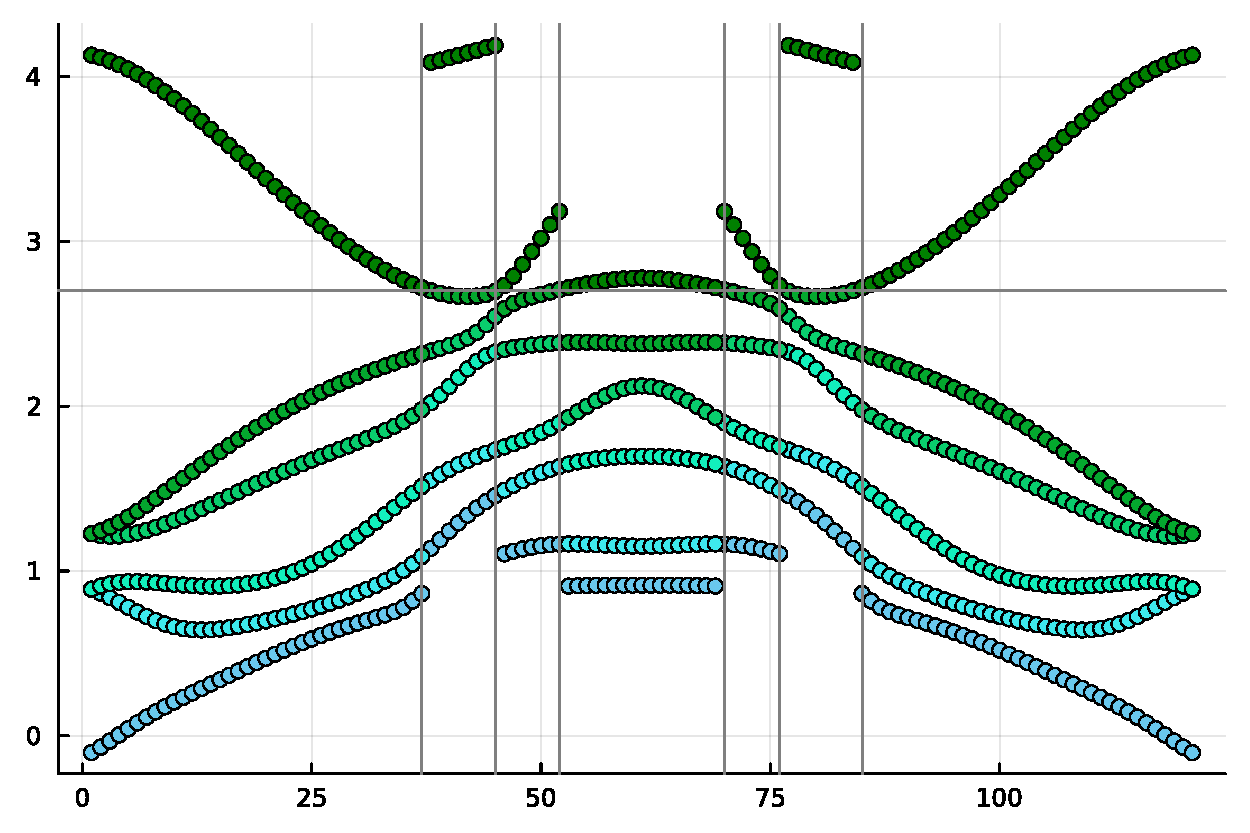
\includegraphics[width=0.5\textwidth]{plots/dft-level-bands.pdf}
    \caption{Example of how \shortcode{inteqp} misidentifies DFT-level bands:
    the data is from the DFT column of \shortcode{eqp.dat};
    the colors of points are about the band index.}
    \label{fig:inteqp-shuffle-band-index-1}
\end{figure}

If the system is metallic in the DFT level 
(regardless of what $GW$ says about the material, 
and the screening model used)
and \shortcode{inteqp} is used, 
this is expected:
somehow, \shortcode{inteqp} assumes the system is an insulator,
and thus states above the Fermi energy (but not too far from it)
has to be in one band.
Thus, if, say, the 120th band has more than one intersection points 
with the Fermi energy level,
its part below $\varphi_{\text{F}}$ will be recognized as the 119th band
in the eyes of \shortcode{inteqp}.
This can be seen by plotting the DFT column of the \shortcode{eqp.dat} output of \shortcode{inteqp}
(\prettyref{fig:inteqp-shuffle-band-index-1}).

\subsection{The size of band gap}\label{sec:band-gap-problem}

DFT is infamous for underestimating the band gap.

\begin{itemize}
    \item Use hybrid functionals like HSE.
    \item Let $GW$ correct the band structure. TODO: but how? How to avoid the error in \prettyref{sec:semimetal-error-1}?
\end{itemize}

\subsection{When we get a semimetal in the DFT step but it should be an insulator}\label{sec:unexpected-metal}

This is similar to \prettyref{sec:band-gap-problem}.

Note that naively feeding the semimetal result into BerkeleyGW 
while still using the insulator procedure
may result in errors in \prettyref{sec:segment-fault-1}. 

One way to solve the problem is 
to manually move the conduction bands and the valence bands away from each other.
Naively using the \shortcode{eqp_correction} option 
and shifting bands near the Fermi surface away from each other 
leads to \prettyref{sec:semimetal-error-1},
precisely because 
``QP corrections'' (i.e. the energy shift manually added by me) 
change the character of some states from valence to conduction.
The \shortcode{mf_header/kpoints/occ} and \shortcode{mf_header/kpoints/ifmax} datasets 
in the \shortcode{WFN.h5} file 
have to be modified accordingly.
TODO: should this be done in \shortcode{2-sigma}?

The problem with this method is we don't have \shortcode{eqp_correction} in \shortcode{kernel}. TODO 

\bibliographystyle{plain}
\bibliography{gw,dft,wannier}

\end{document}